% --------------------------------------------------------------------------- %
% --------------------------------------------------------------------------- %
\chapter{Background Estimates}
\label{ch:bkgs}

\section{Types of Backgrounds}
\label{sec:bkgs}
The \mttwo all-hadronic search is primarily a search for missing energy, and the backgrounds present in the signal region can be roughly categorized into two groups: events with ``fake'' missing energy due to mismeasurement of energies or other experimental effects, and those with``real'' missing energy due to the underlying physics process which escapes the detector. In this analysis, the primary backgrounds from SM processes with \MET and hadronic activity in the final state can be divided into three categories:
\begin{itemize}
	\item {\it Multijet events}, with no true missing energy generating fake \MET. Such all-hadronic events usually enter analysis signal regions due to mismeasurement of jet energy or sporadic noise.
	\item {\it Lost lepton events}, with a lepton in the final state that is either not identified, reconstructed, in the fiducial region of the detector, or sufficiently isolated to pass the lepton selections. The bulk of these events are due to leptonic W boson or top quark decays (which may also produce significant real \MET with an associated neutrino) recoiling against jets.
	\item {\it Invisible Z events}, where a Z boson produced in association with jets decays into neutrinos. The neutrinos are extremely weakly interacting particles which escape the detector without leaving any signature, and so this background is fundamentally very similar to many of the BSM signals which may appear in each search region. It is a dominant background in many signal regions, though the relative fraction decreases in regions with more b-tagged jets (\nb).
\end{itemize}

In order to provide a robust prediction of each background that is not heavily dependent on simulation alone, each background is estimated using data-driven techniques as described in the following sections. The control regions for each background can be found in chapter \ref{ch:analysis}.

% --------------------------------------------------------------------------- %
% --------------------------------------------------------------------------- %
\section{Multijet Estimate}
\label{sec:qcd}

The estimate of the SM multijet background utilizes two different techniques depending on the number of jets in a given signal region. For regions with two or more jets, the background is estimated by extrapolating to regions with high \dphimin after inverting the \dphimin requirement. In the monojet signal regions, a sample enriched in unbalanced dijet events is used to extrapolate to regions with low sub-leading jet momentum.

\subsection{Multijet Signal Region Prediction}
\label{subsec:qcdMultijet}

As outlined in section \ref{subsec:multijetCR}, the multijet background in control regions with two or more jets is estimated using a QCD-enriched sample where \HT triggers are used to select events with an inverted \dphimin cut. The ratio of events with high to low \dphimin (\rphi) is modeled as a power law function in \mttwo, as shown in equation \ref{eq:rphi}. 
\begin{equation}
	r_{\phi}(\mttwomath) = \frac{N(\dphiminmath > 0.3)}{N(\dphiminmath < 0.3)} = a \cdot M_{\mathrm{T2}}^b
	\label{eq:rphi}
\end{equation}

The power-law dependence of \rphi on \mttwo is verified in simulation for events with $\mttwomath > 60 \GeV$,, as illustrated in figure \ref{fig:rphiDependence}. Because the dominant source of \MET in low \mttwo events is not necessarily due to jet mismeasurement, the fit is performed in the window $60 < \mttwomath < 100 \GeV$ except in extreme \HT regions where a lower bound of 70\GeV is used (as a conservative measure since these regions have high statistics). The upper bound of 100 \GeV is chosen such that the contamination of electroweak and top-quark events is small compared to the QCD multijet yield. A systematic uncertainty in the \rphi value is assigned based on variations of the fit window, by shifting the lower boundary of the window in either direction while preserving the fit statistics by shifting the upper boundary of the window. The systematic uncertainty is then taken as the maximal deviation of all such variation with respect to the nominal window.
\begin{figure}
	\centering
	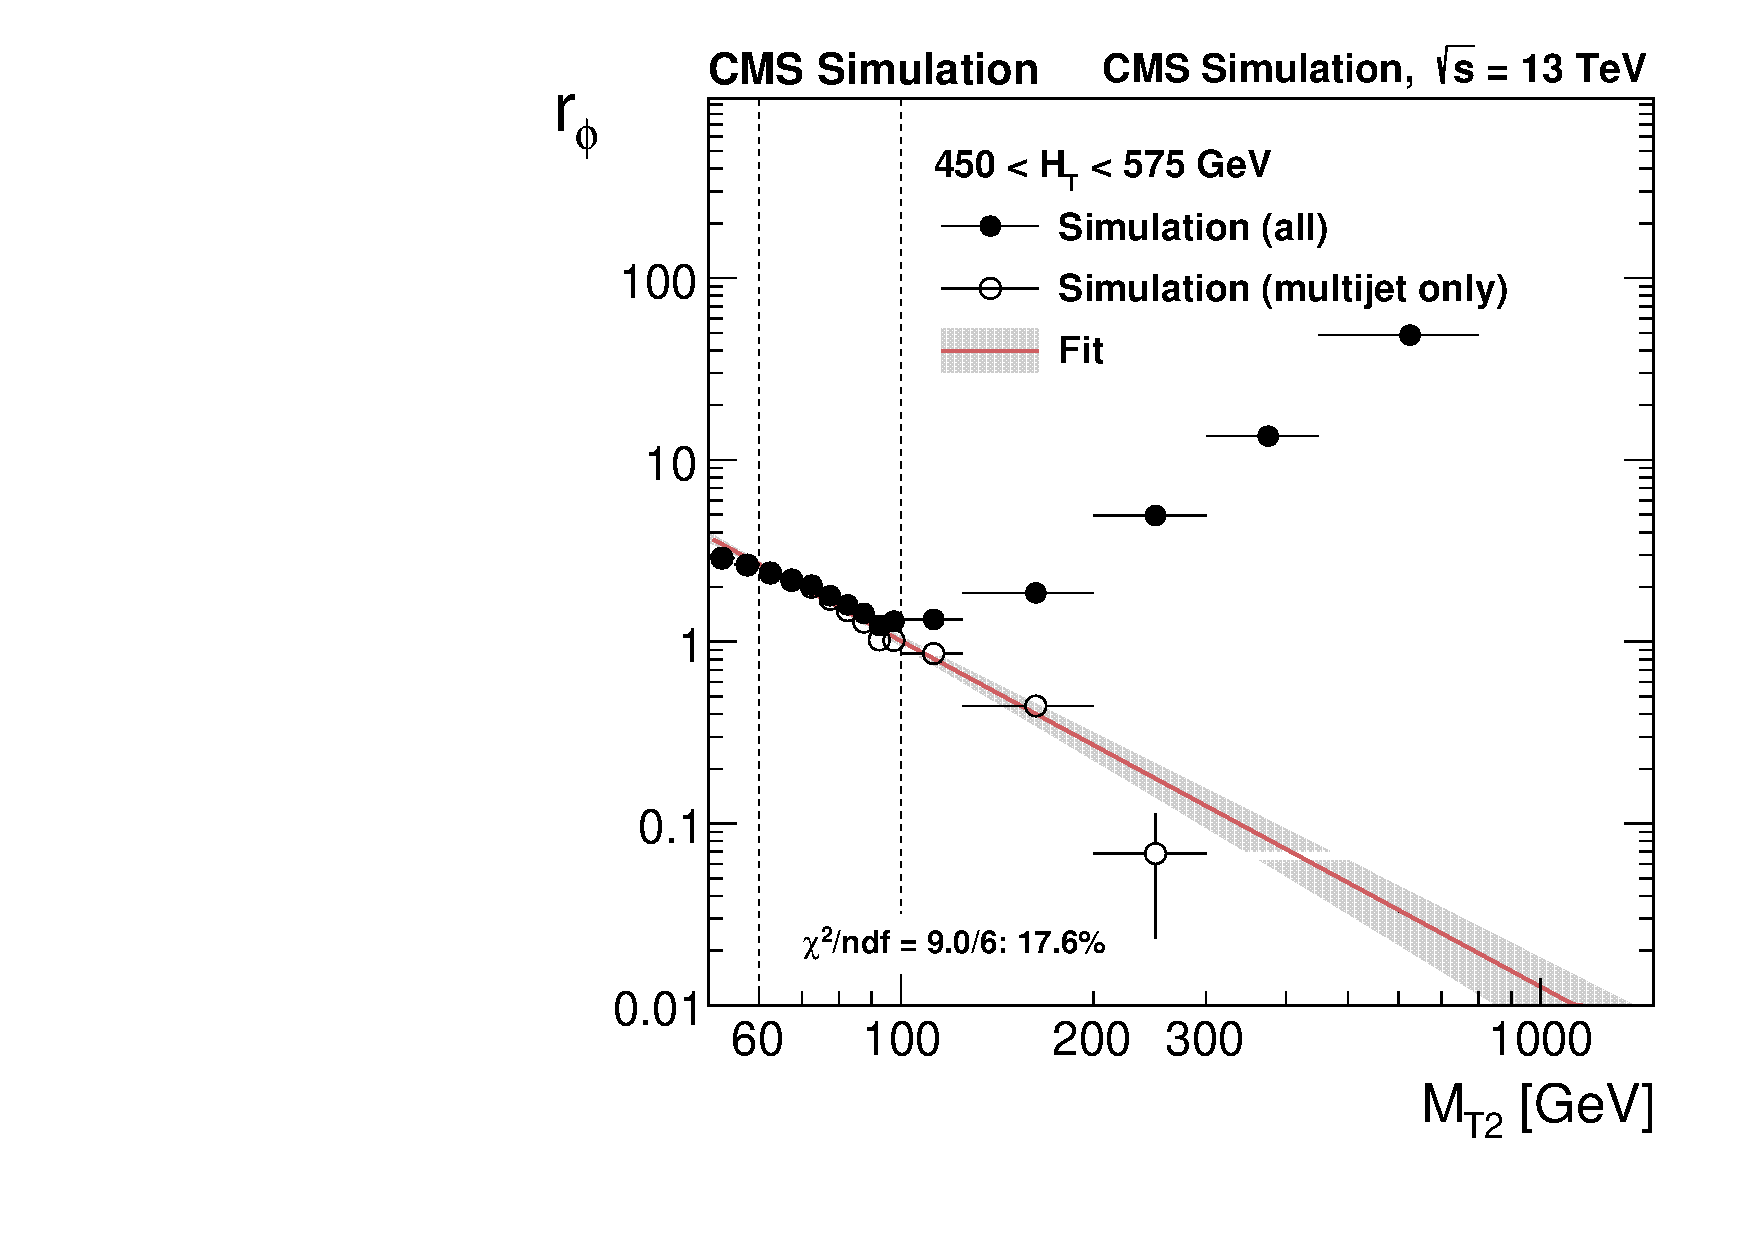
\includegraphics[width=0.35\textwidth]{backgrounds/figs/ratio_HT450to575_j2toInf_b0toInf}
	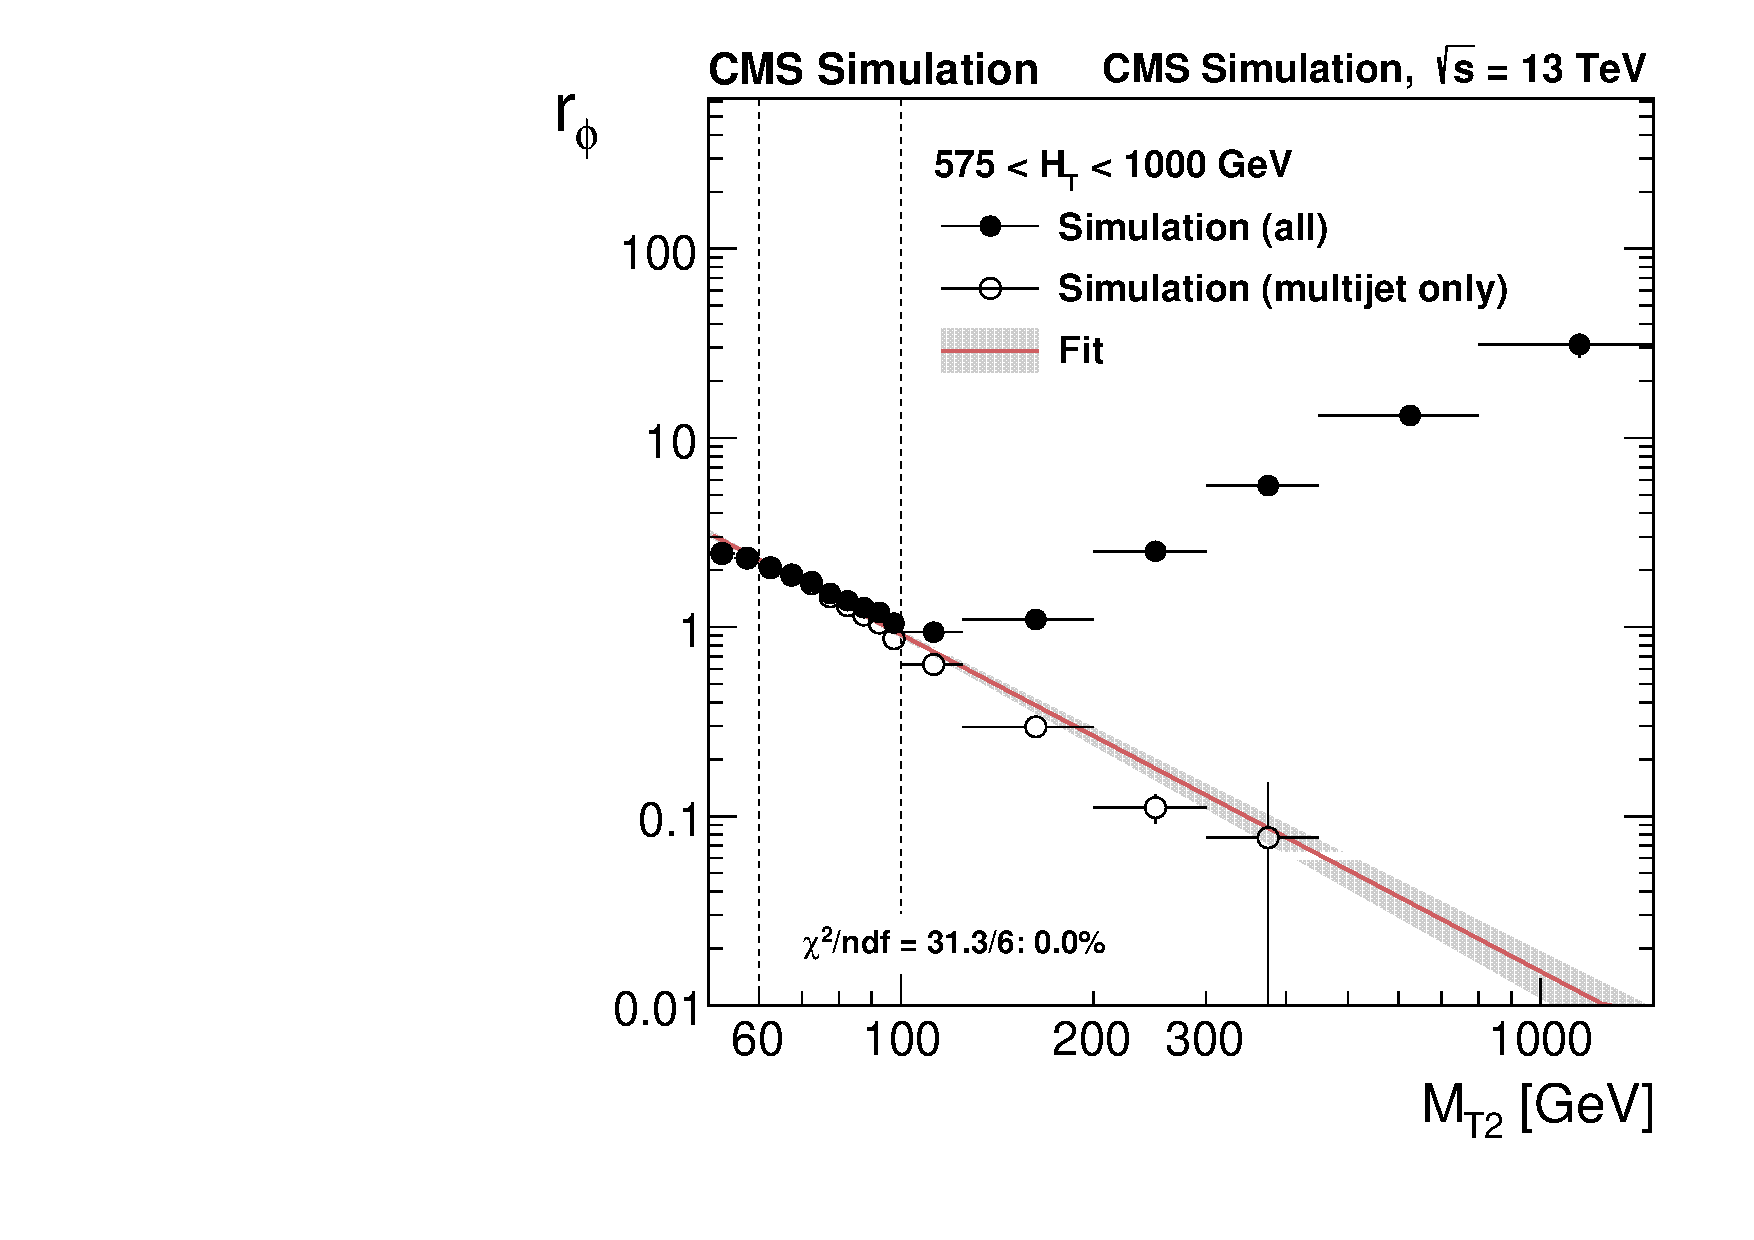
\includegraphics[width=0.35\textwidth]{backgrounds/figs/ratio_HT575to1000_j2toInf_b0toInf}
	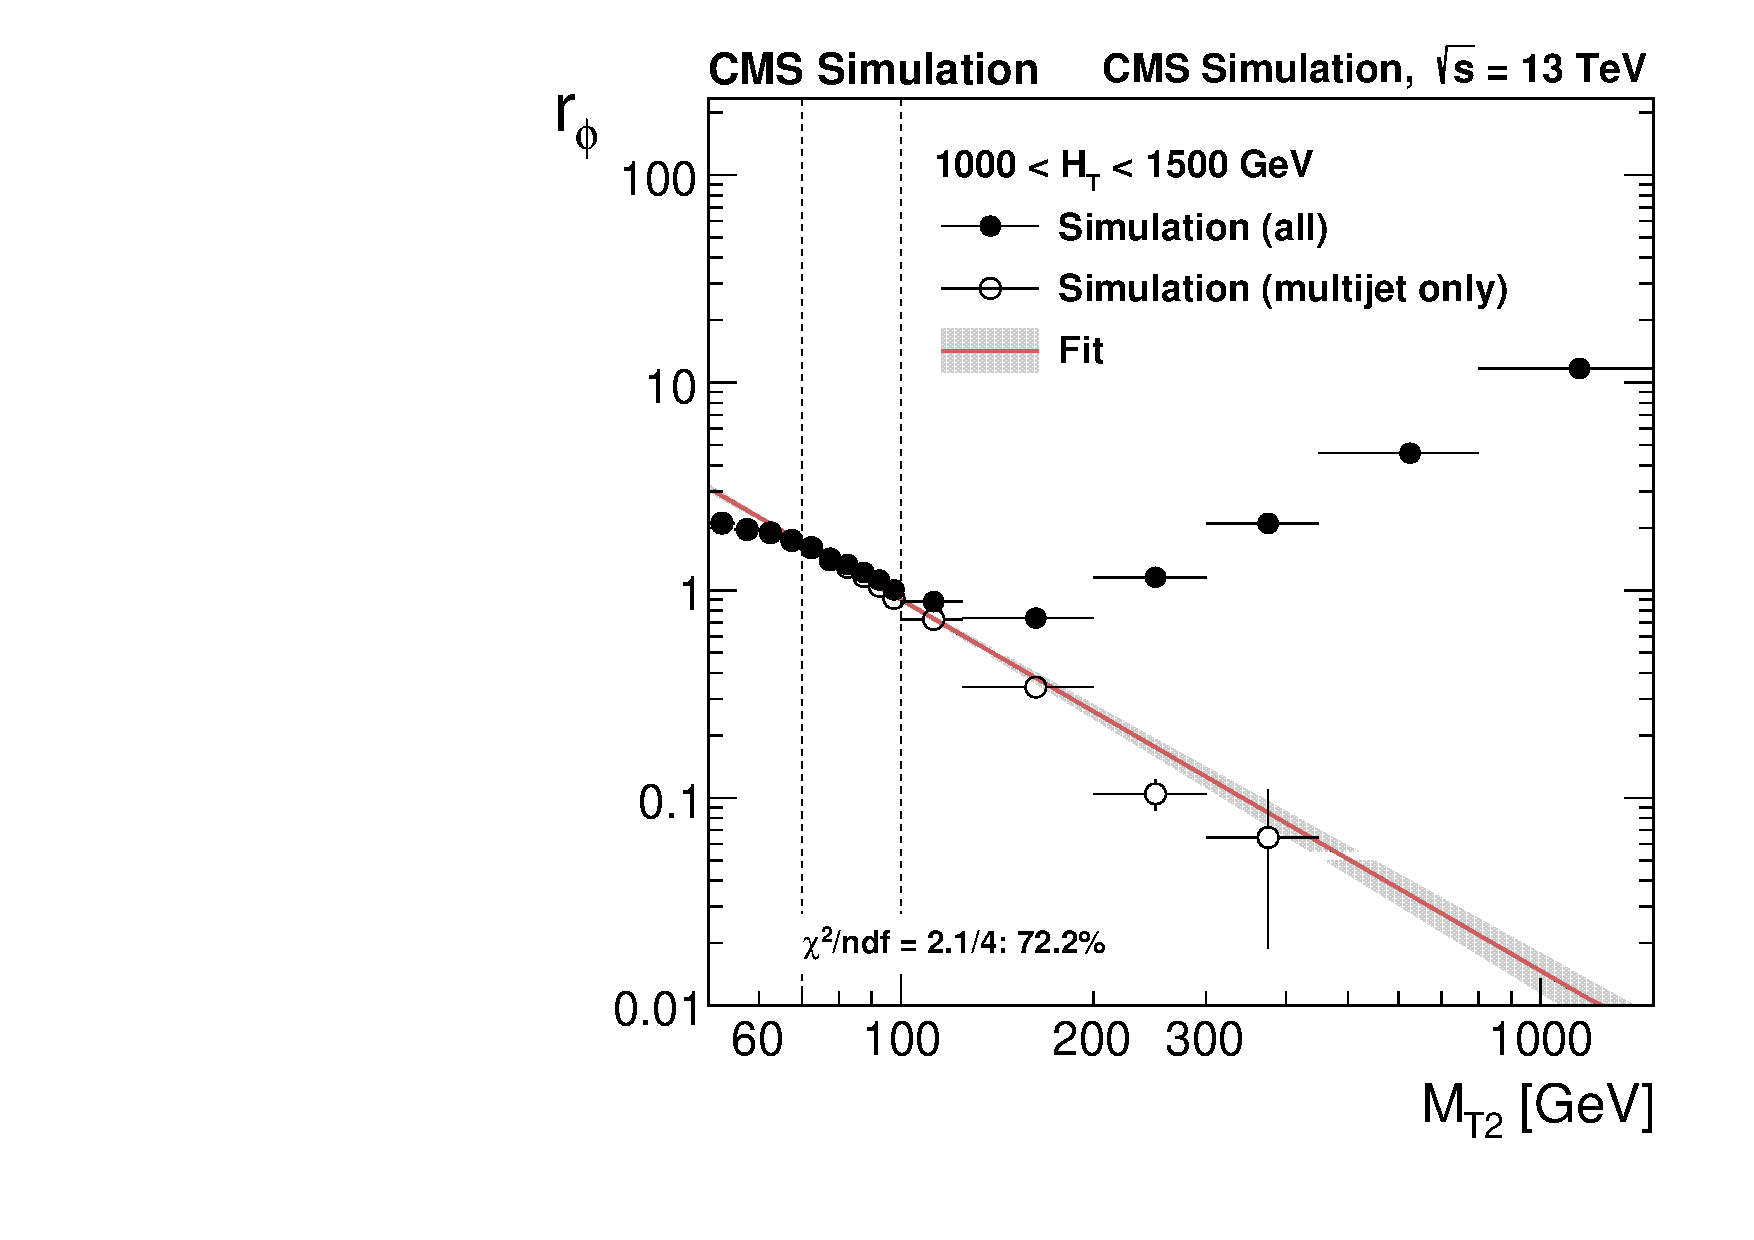
\includegraphics[width=0.35\textwidth]{backgrounds/figs/ratio_HT1000to1500_j2toInf_b0toInf}
	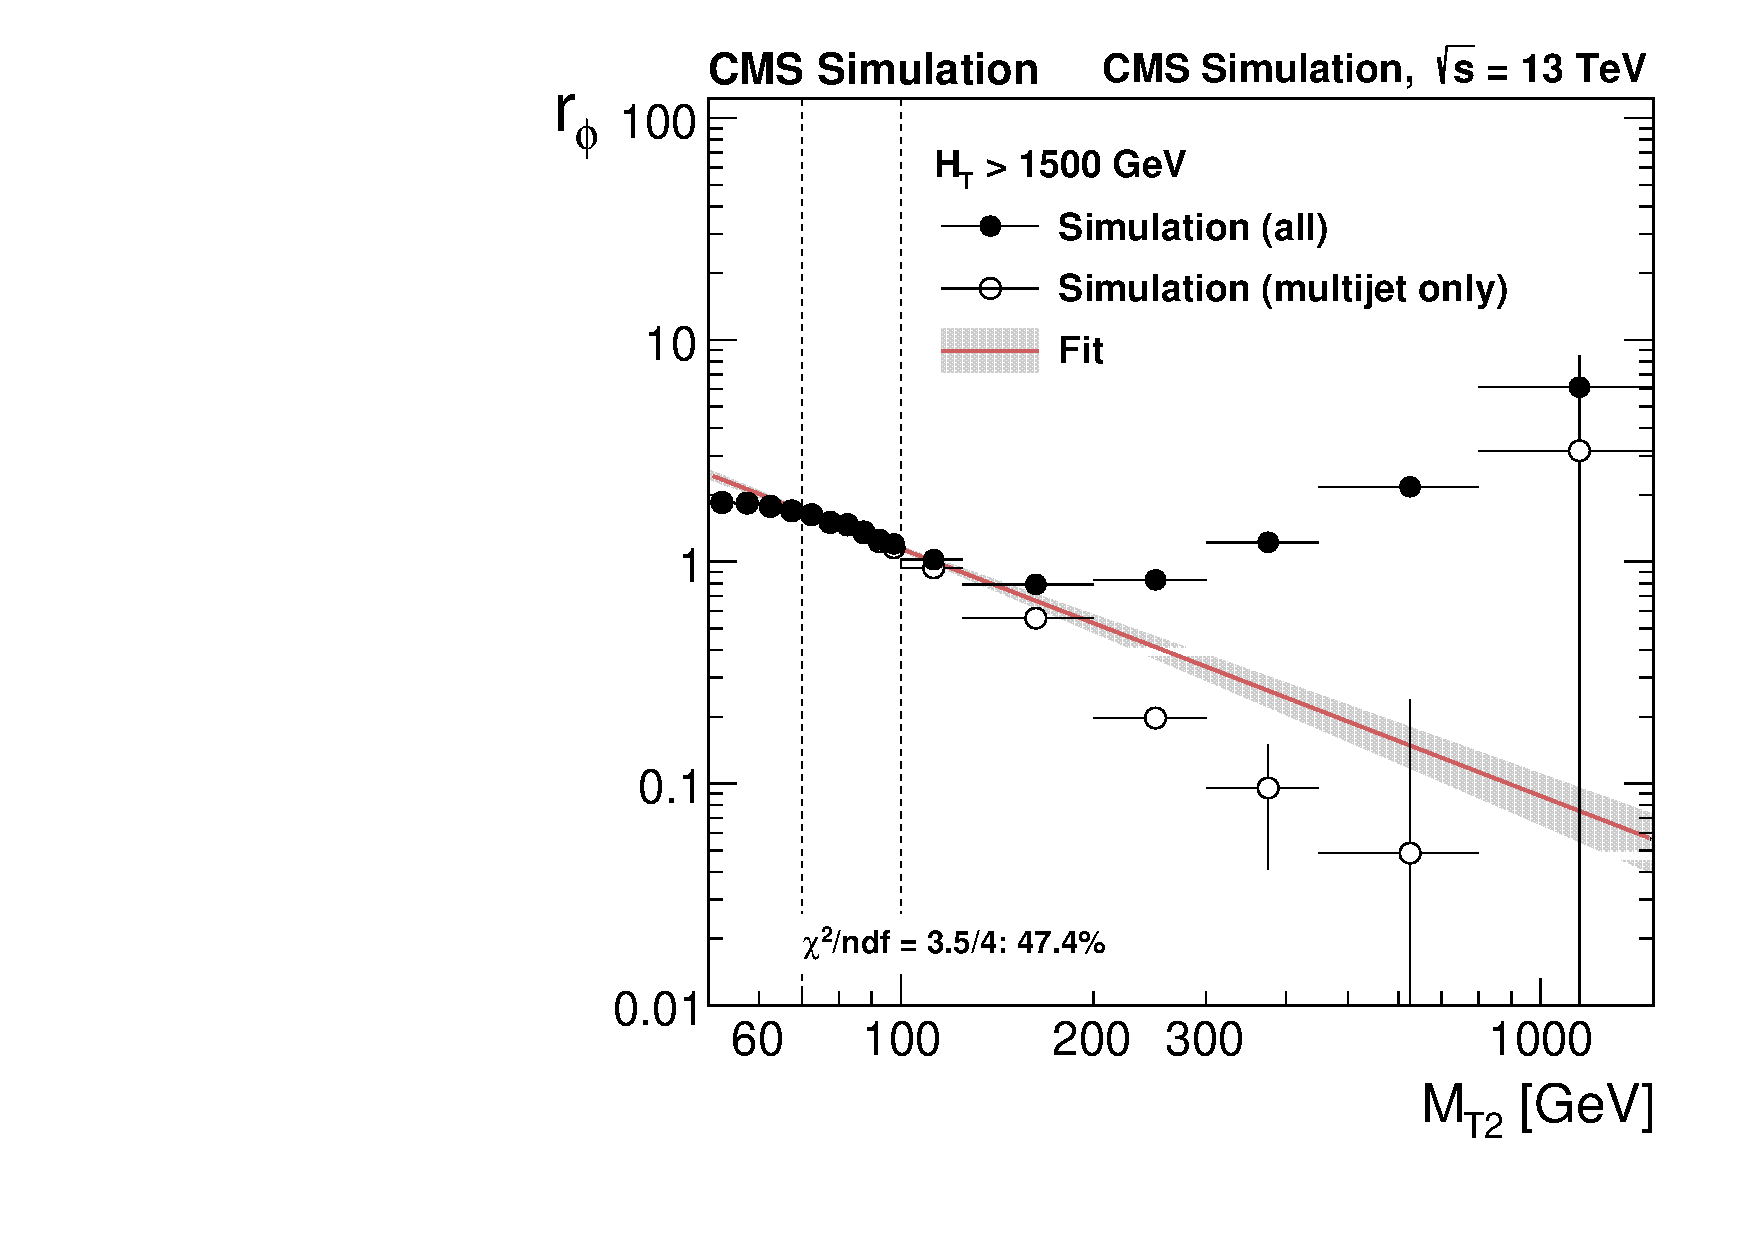
\includegraphics[width=0.35\textwidth]{backgrounds/figs/ratio_HT1500toInf_j2toInf_b0toInf}
	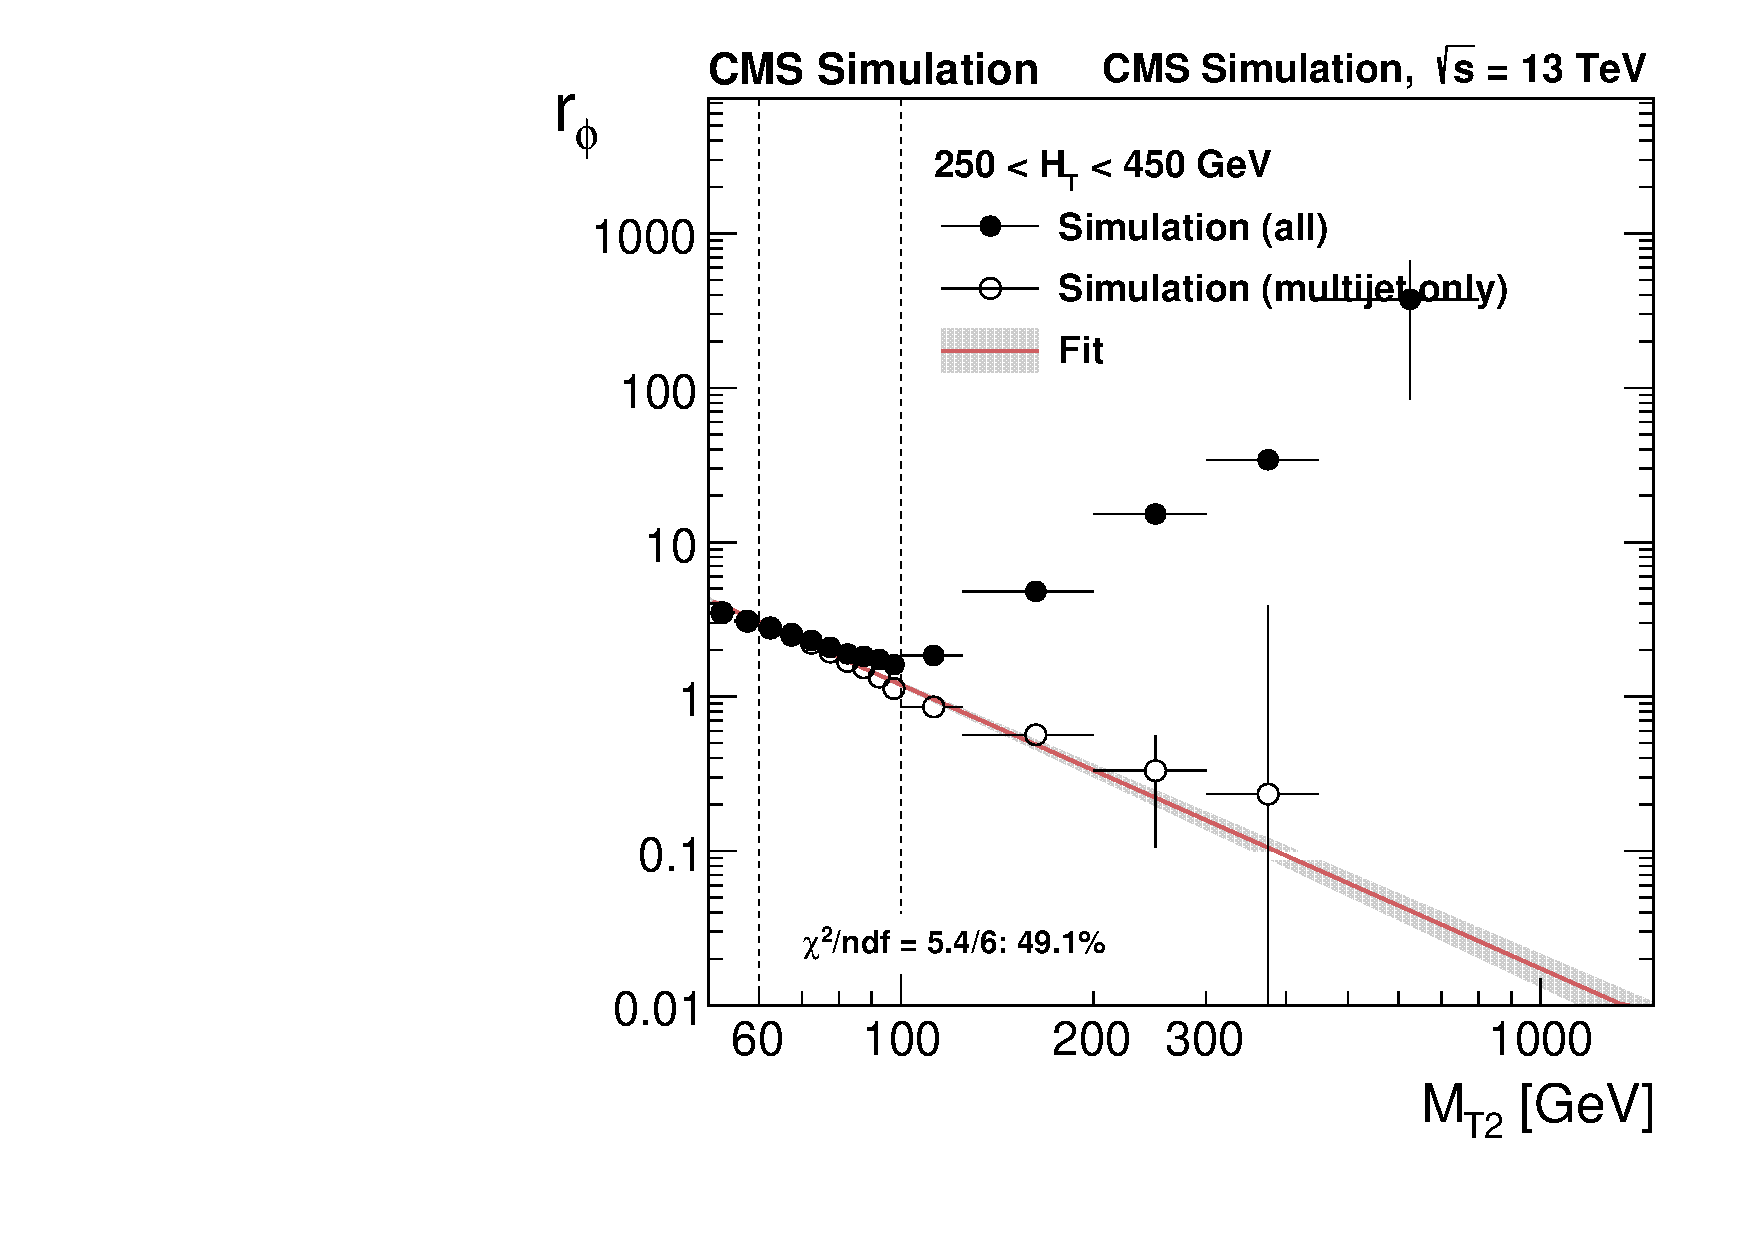
\includegraphics[width=0.35\textwidth]{backgrounds/figs/ratio_HT250to450_j2toInf_b0toInf}
	\caption{Simulated distribution of the \rphi ratio as a function of \mttwo for the low (top left), medium (top right), high (medium left), extreme (medium right), and very low (bottom) \HT regions. Solid points represent the total simulated background, and hollow points show the QCD multijet contribution only. The red line and grey error band illustrates the best fit to a power law function performed in the dashed line fit window}
	\label{fig:rphiDependence}
\end{figure}

Due to the the total integrated luminosity available and the deliberate suppression rate with which some \HT triggers save events (known as the trigger {\it prescale}), the statistics are sufficient to perform fits in \HT regions inclusive in \nj and \nj. The inclusive multijet background estimate can be determined using \rphi as a function of \mttwo $N_{\mathrm{inc}}^{SR} = r_\phi (\mttwomath) \cdot N_{\mathrm{inc}}^{CR} (\mttwomath)$. The final estimate in a given \nj-\nb bin can be determined as in equation \ref{eq:qcdEstimate}, where \fj is the fraction of multijet events in bin \nj in a given \HT bin, and \rb is the ratio of events with \nb b-tags in a given \nj bin. 
\begin{equation}
	N_{j,b}^{SR}(\mttwomath) = r_\phi (\mttwomath) \cdot N_{\mathrm{inc}}^{CR} (\mttwomath) \cdot f_j (H_{\mathrm{T}}) \cdot r_b (N_{\mathrm{jets}}) 
	\label{eq:qcdEstimate}
\end{equation}

The values of \fj and \rb are measured in data using QCD-enriched regions with an inverted \dphi requirement and $100 < \mttwomath < 200$. Based on simulation, \fj and \rb do not significantly depend on \mttwo, and \rb is independent of \HT. Since \fj is dependent on \HT and \rb on \nj, different values of \fj are measured in each inclusive \HT region, and different values of \rb are measured in in inclusive \nj regions. Figures \ref{fig:fj} and \ref{fig:rb} illustrates the data-driven values of \fj and \rb respectively, along with a comparison to simulation. The robustness of invariance with respect to \mttwo and \dphi (and \HT for \rb) is calculated by making several variations of the aforementioned variables and measuring consequent variations in \fj and \rb, and is summarized in table \ref{tbl:fjrbSyst}.

\begin{figure}
	\centering
	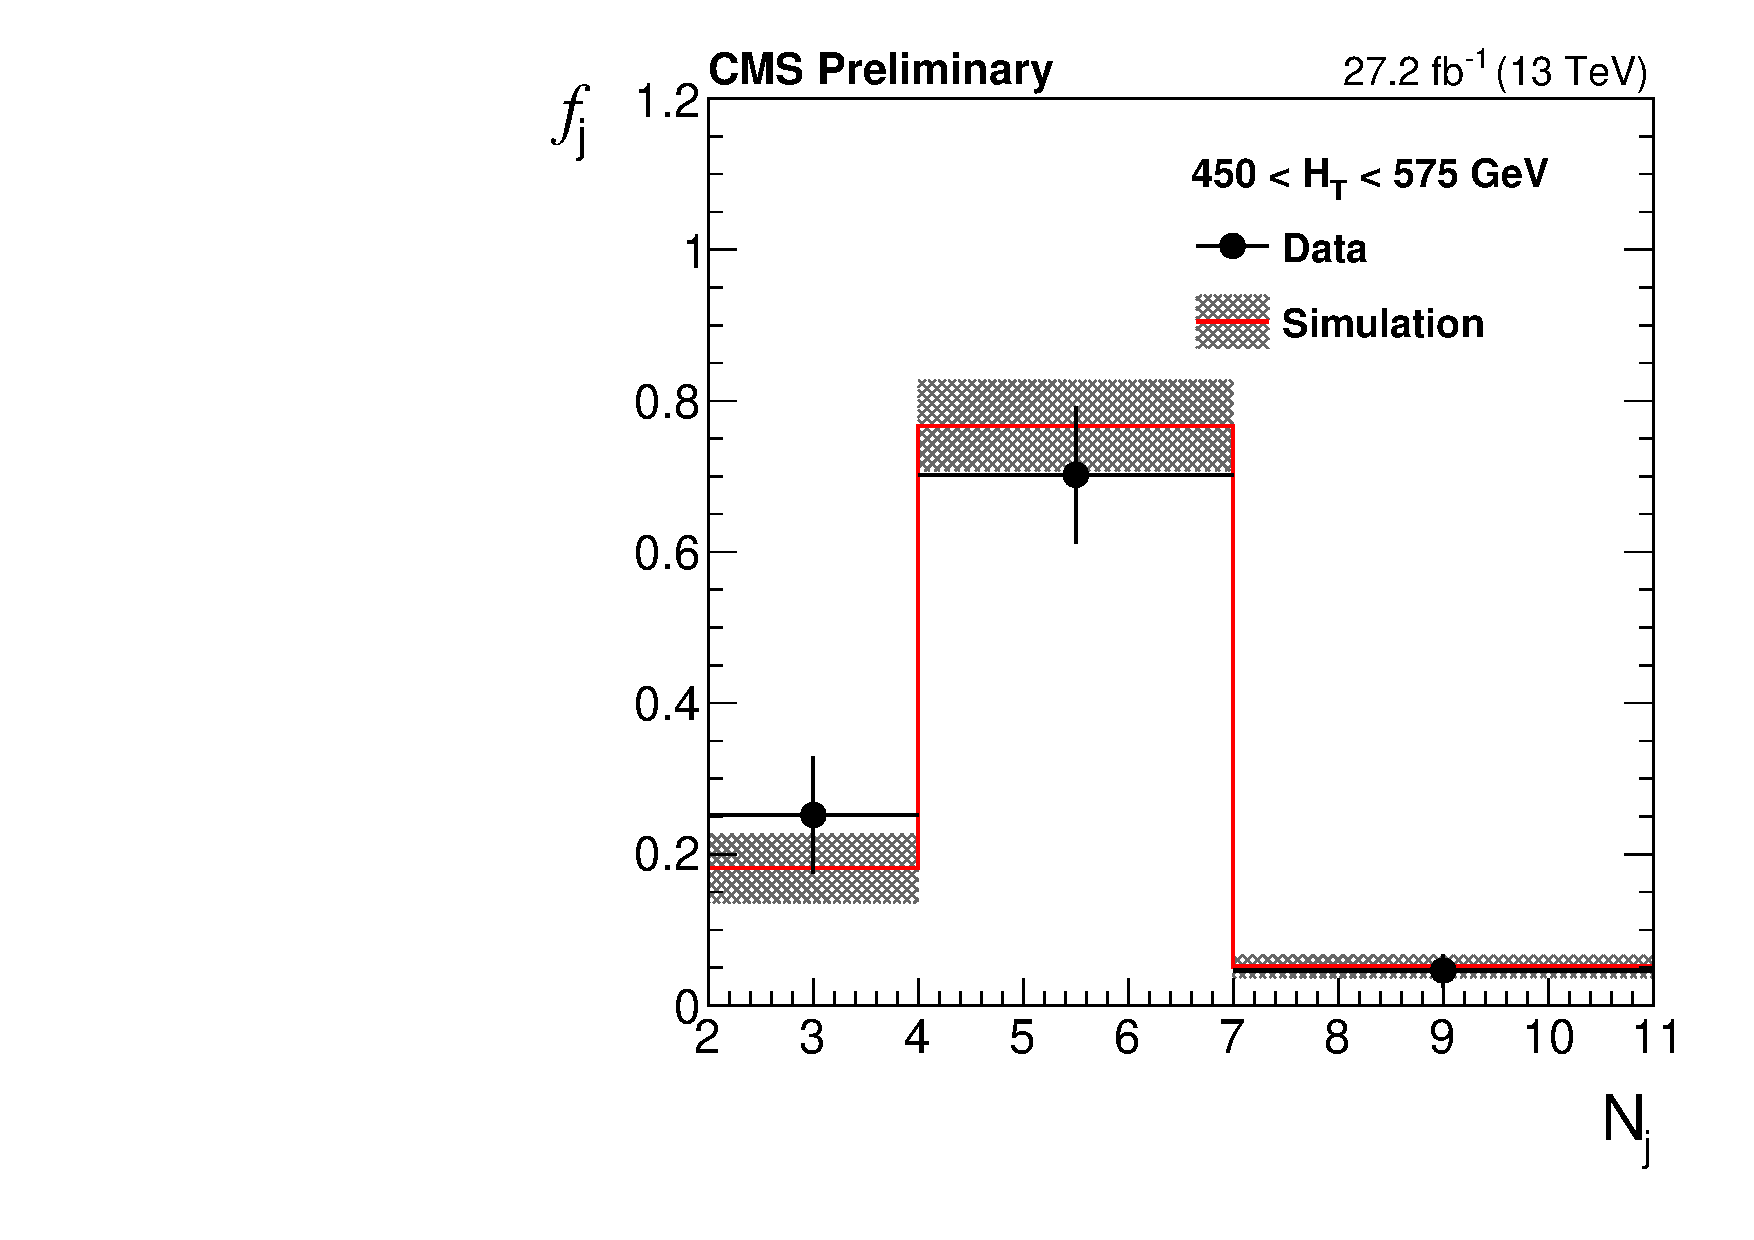
\includegraphics[width=0.35\textwidth]{backgrounds/figs/f_jets_HT450to575_j2toInf_b0toInf}
	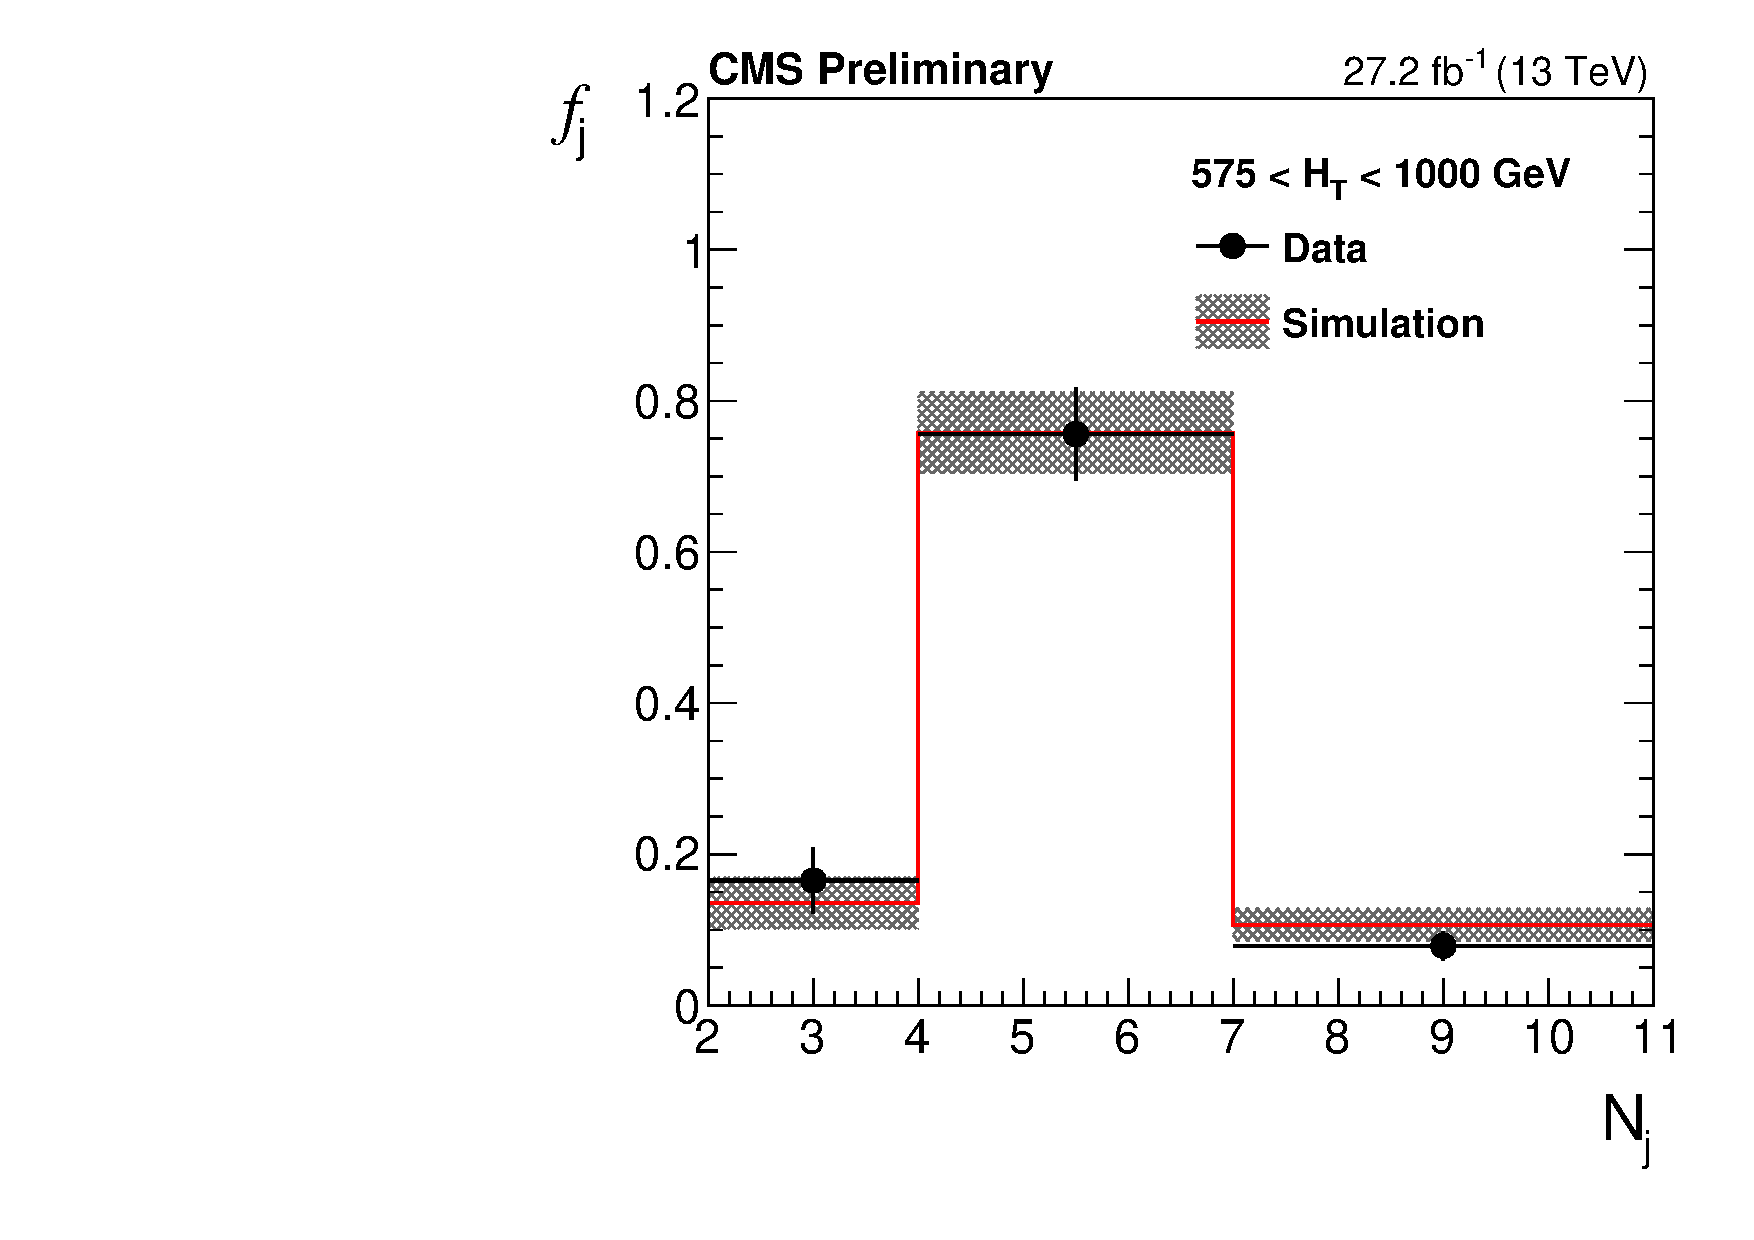
\includegraphics[width=0.35\textwidth]{backgrounds/figs/f_jets_HT575to1000_j2toInf_b0toInf}
	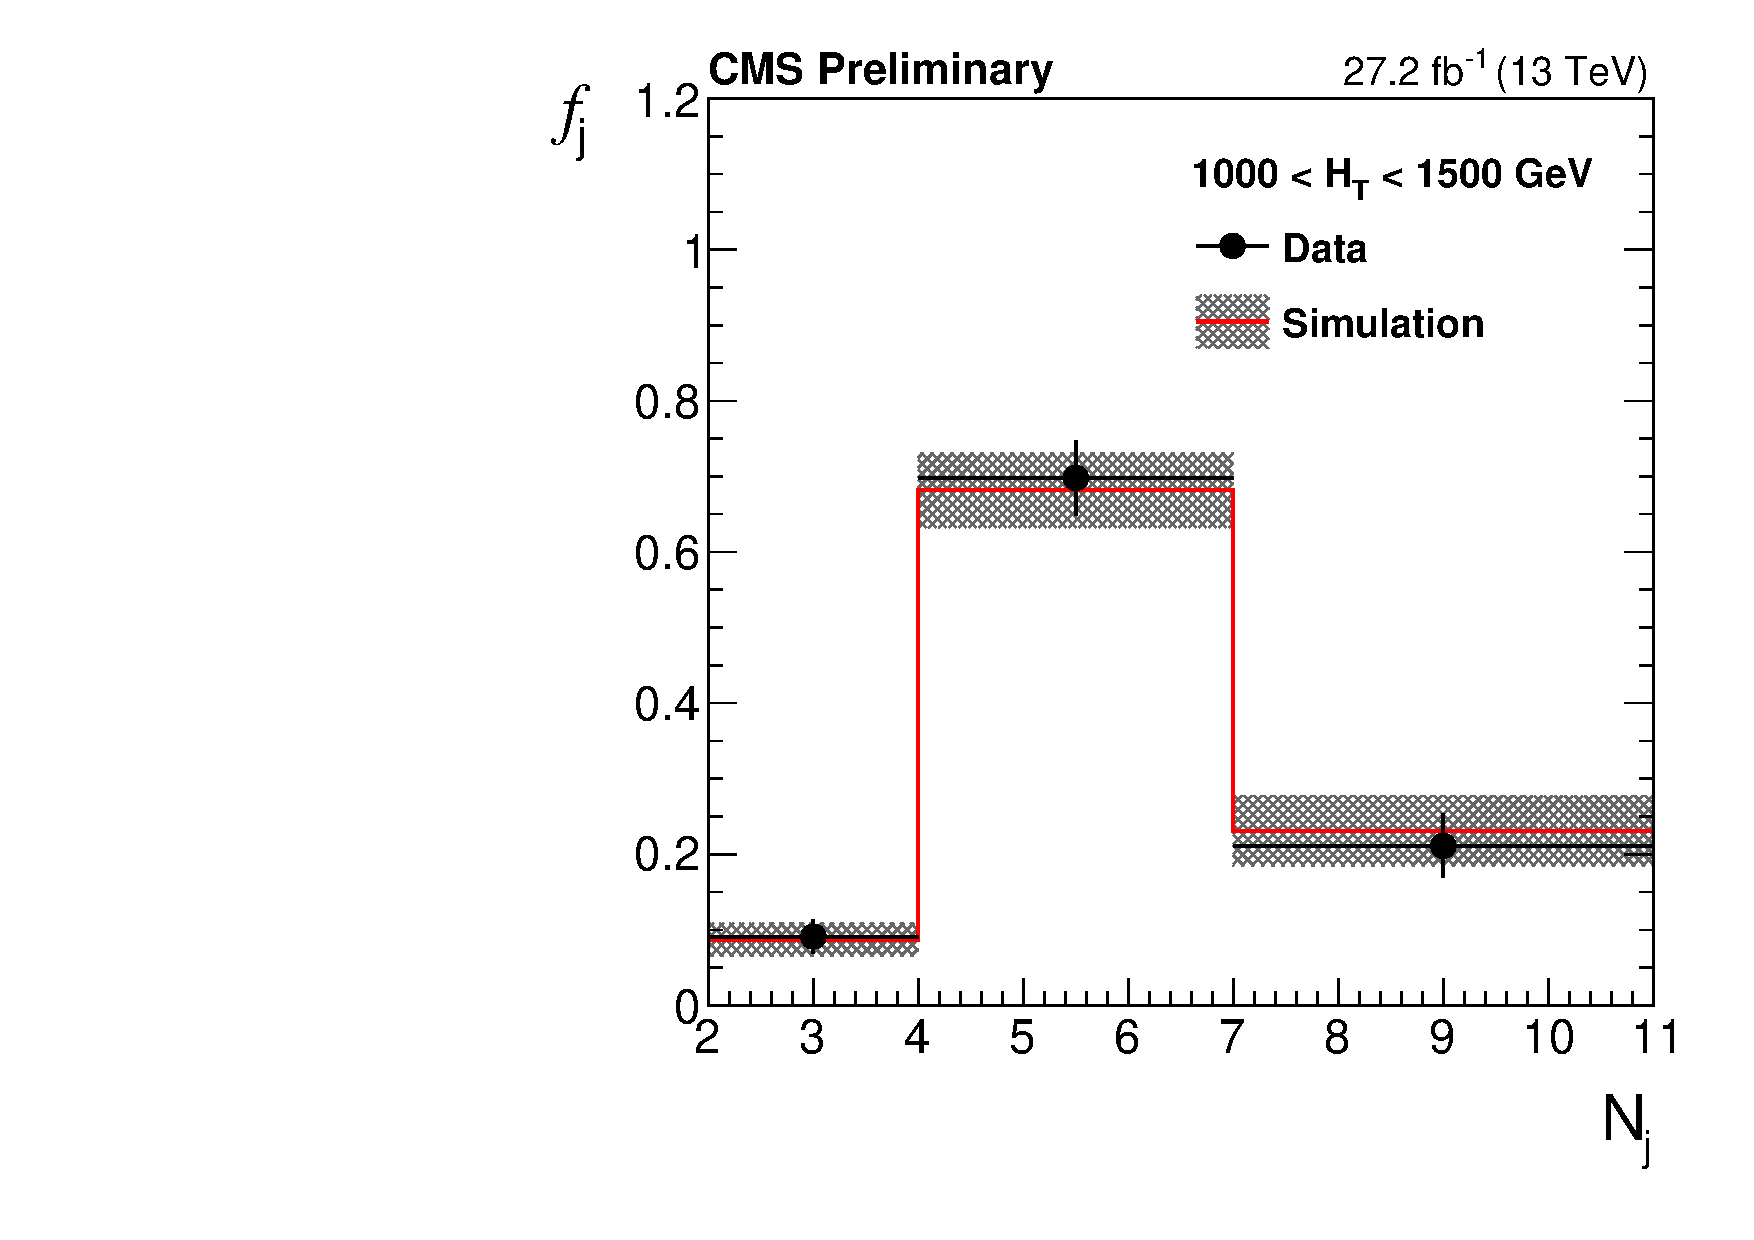
\includegraphics[width=0.35\textwidth]{backgrounds/figs/f_jets_HT1000to1500_j2toInf_b0toInf}
	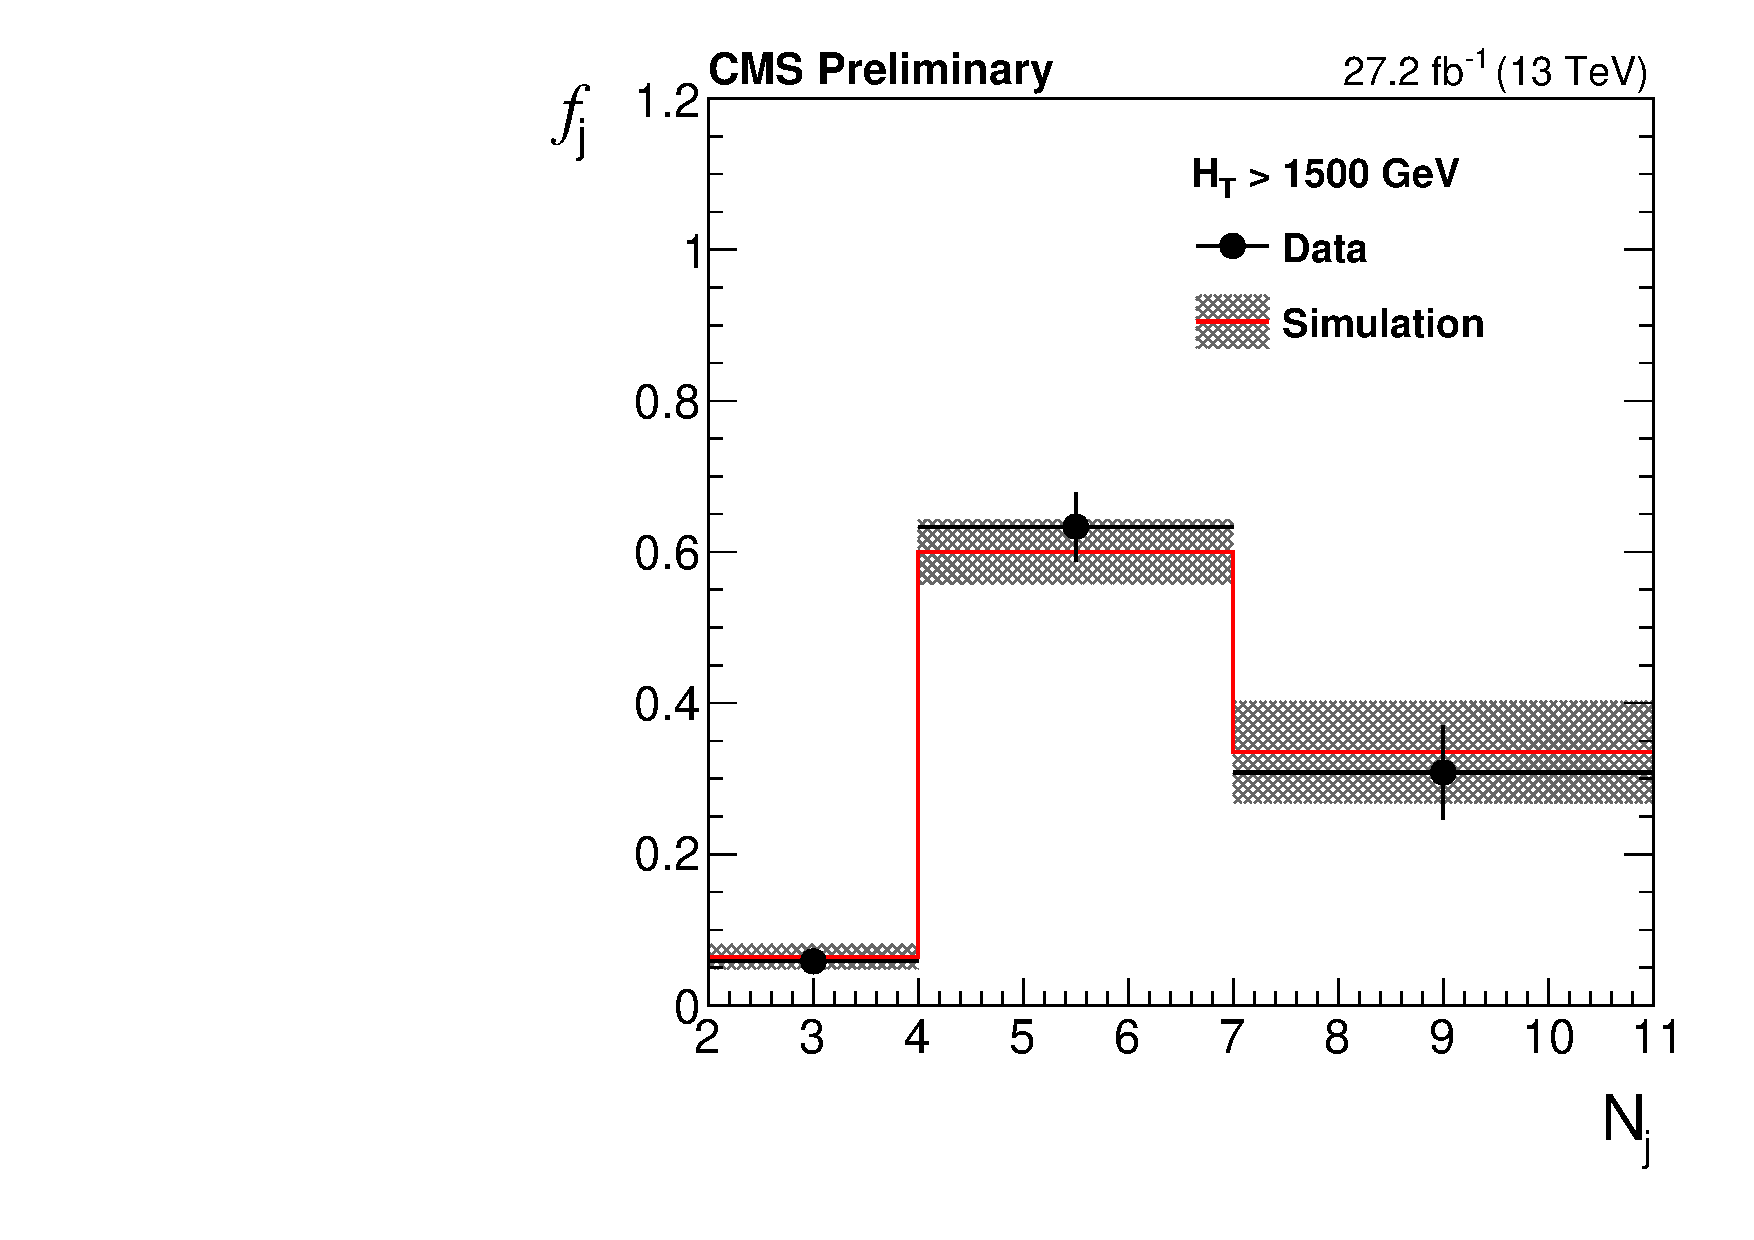
\includegraphics[width=0.35\textwidth]{backgrounds/figs/f_jets_HT1500toInf_j2toInf_b0toInf.pdf}
	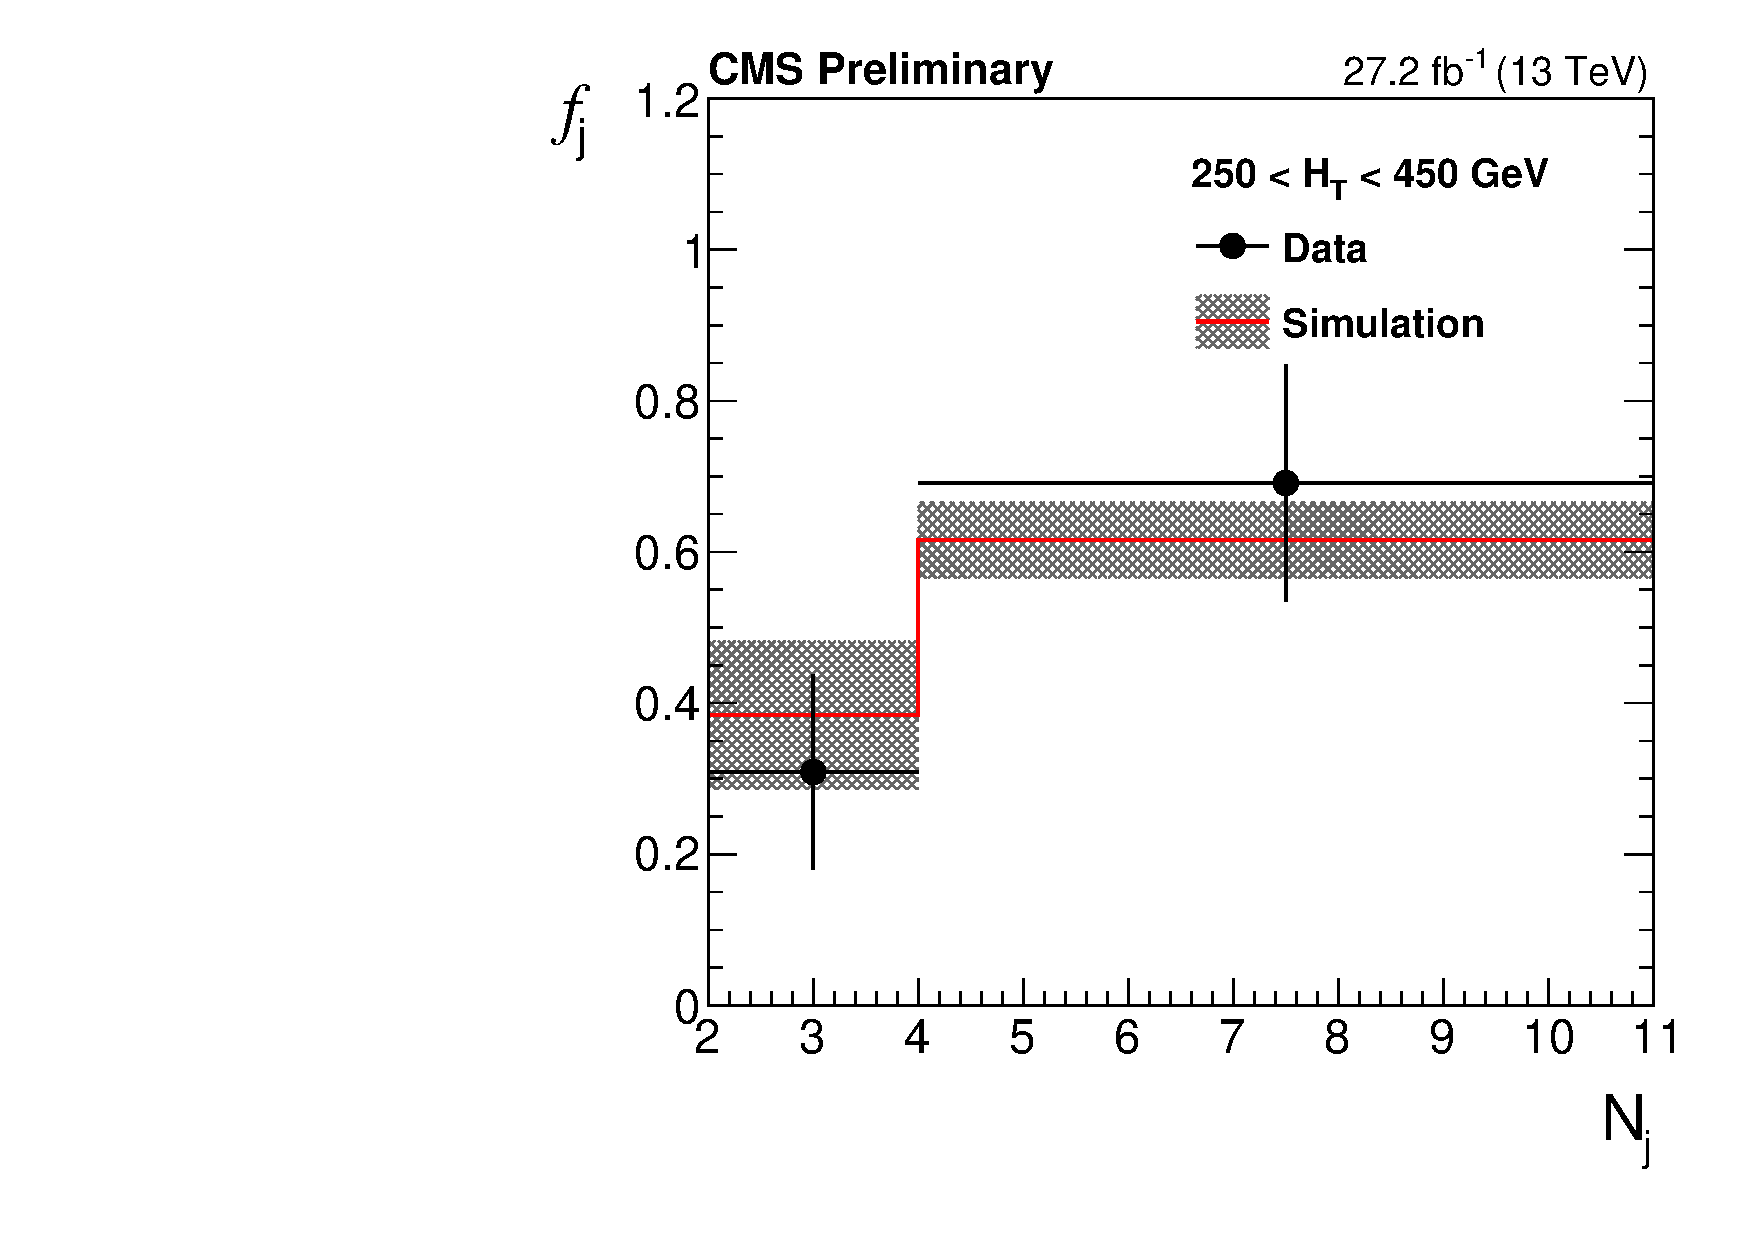
\includegraphics[width=0.35\textwidth]{backgrounds/figs/f_jets_HT250to450_j2toInf_b0toInf}
	\caption{The values of \fj as measured in data in different \HT regions, compared to simulation. The uncertainties include both the statistical error and the systematic sources as listed in table \ref{tbl:fjrbSyst}}
	\label{fig:fj}
\end{figure}
\begin{figure}
	\centering
	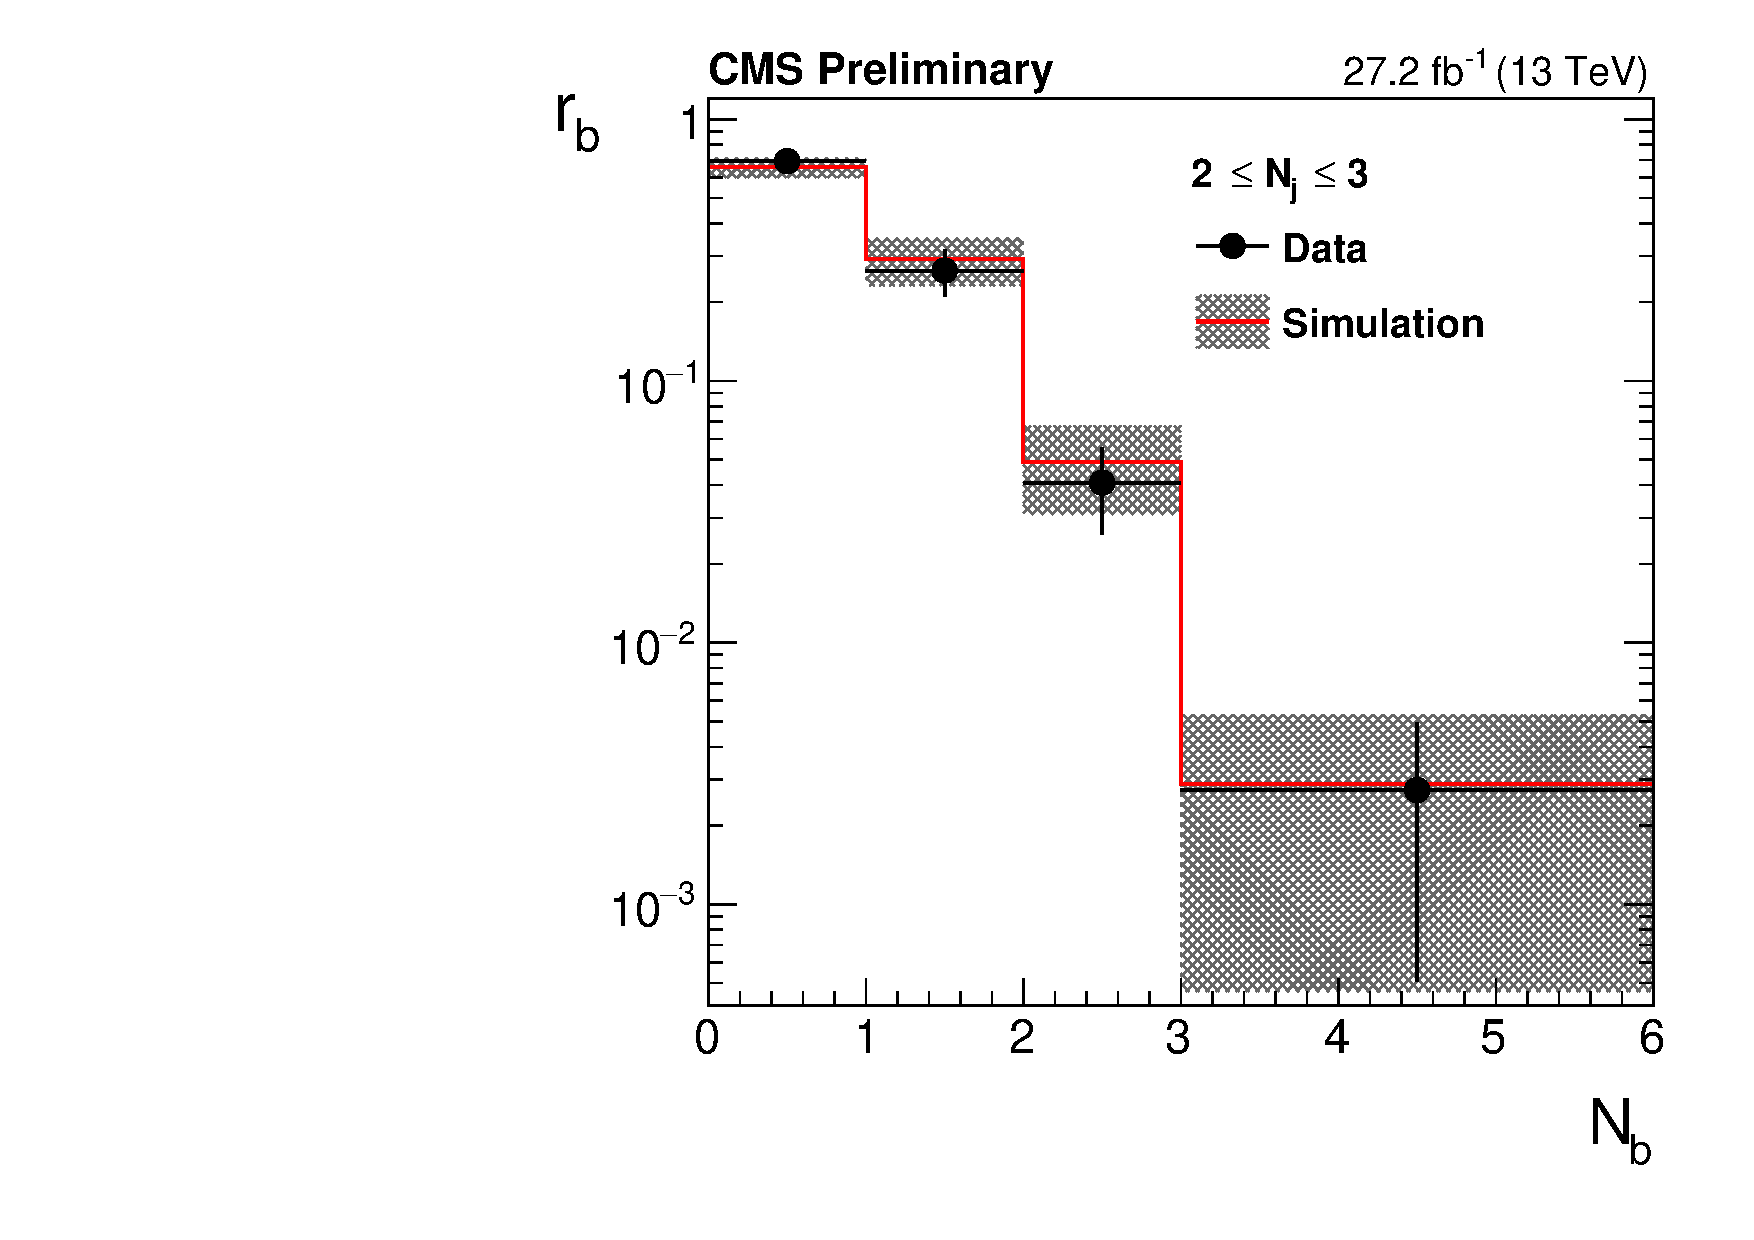
\includegraphics[width=0.45\textwidth]{backgrounds/figs/r_hat_HT250toInf_j2to3_b0toInf}
	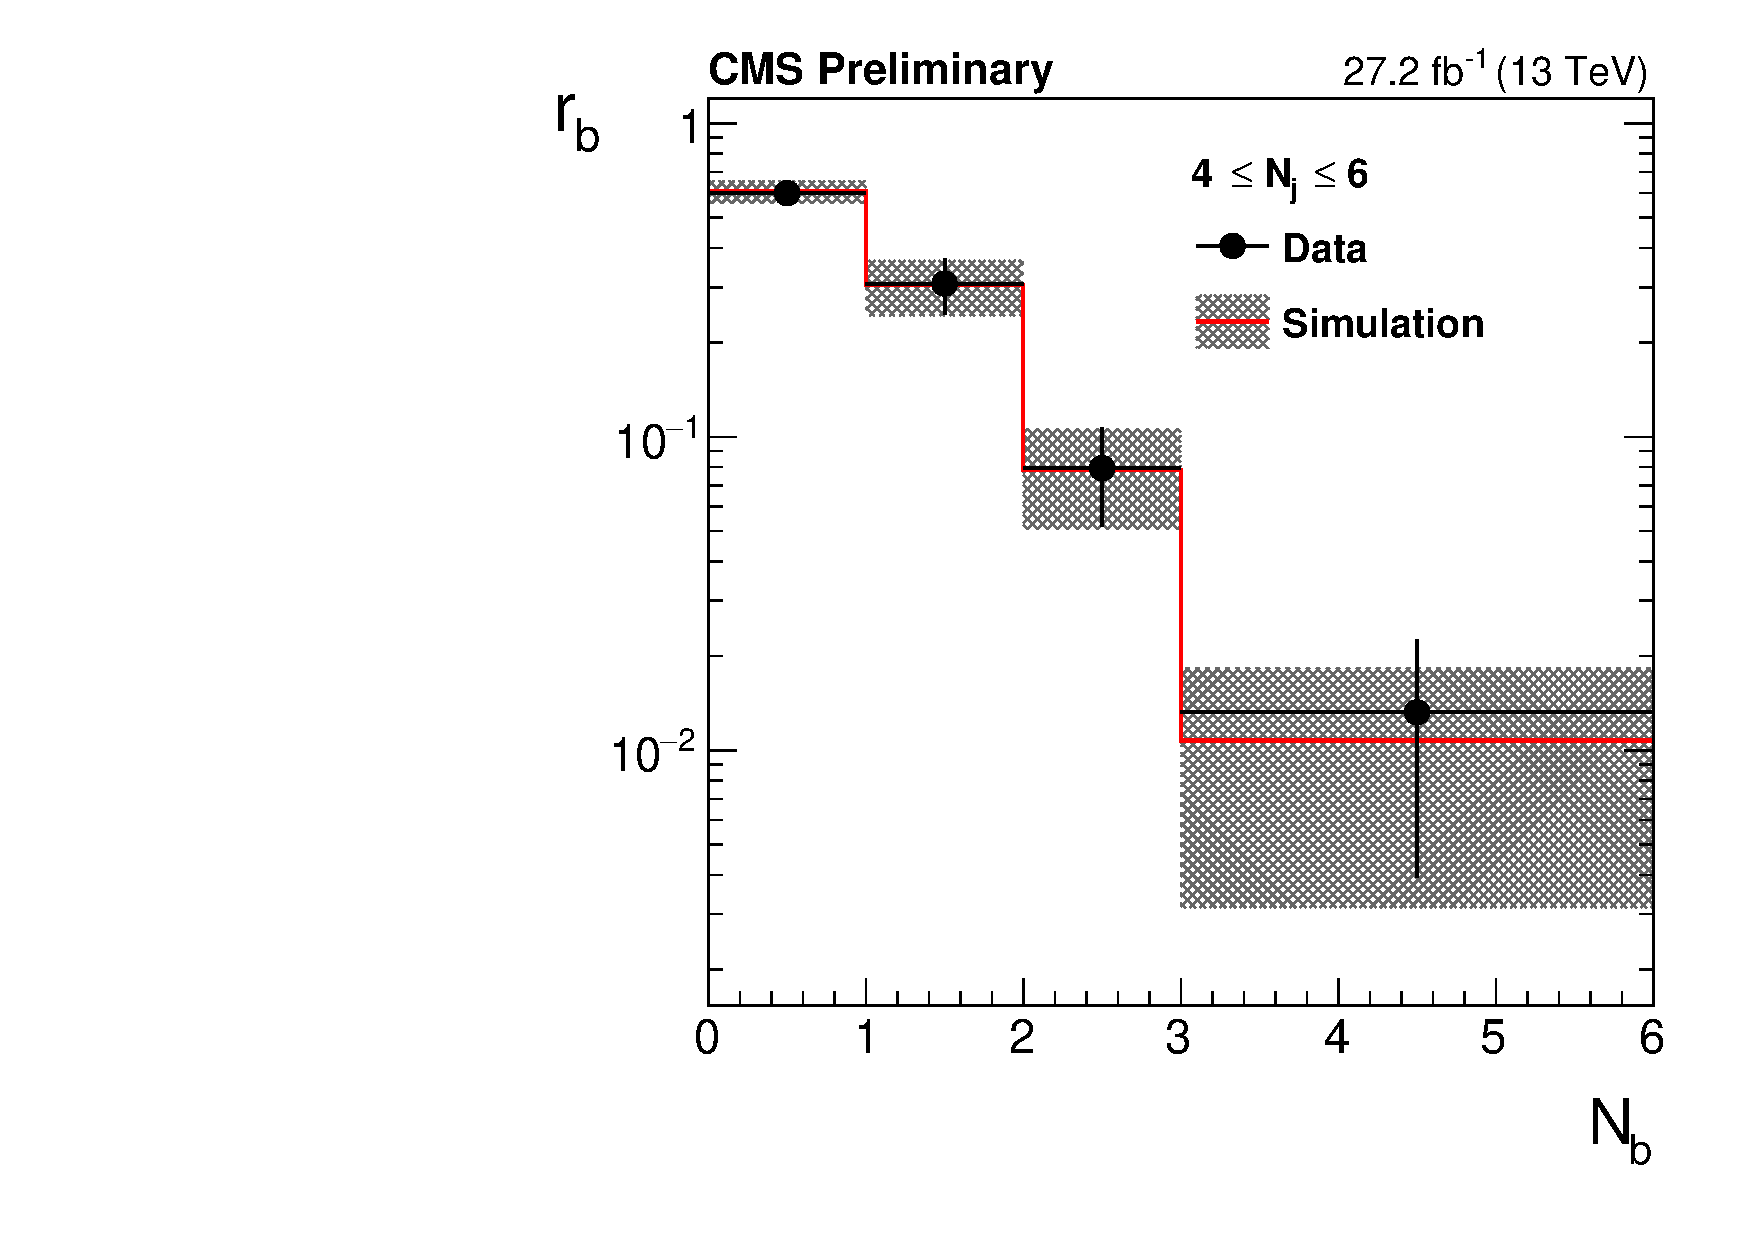
\includegraphics[width=0.45\textwidth]{backgrounds/figs/r_hat_HT250toInf_j4to6_b0toInf}
	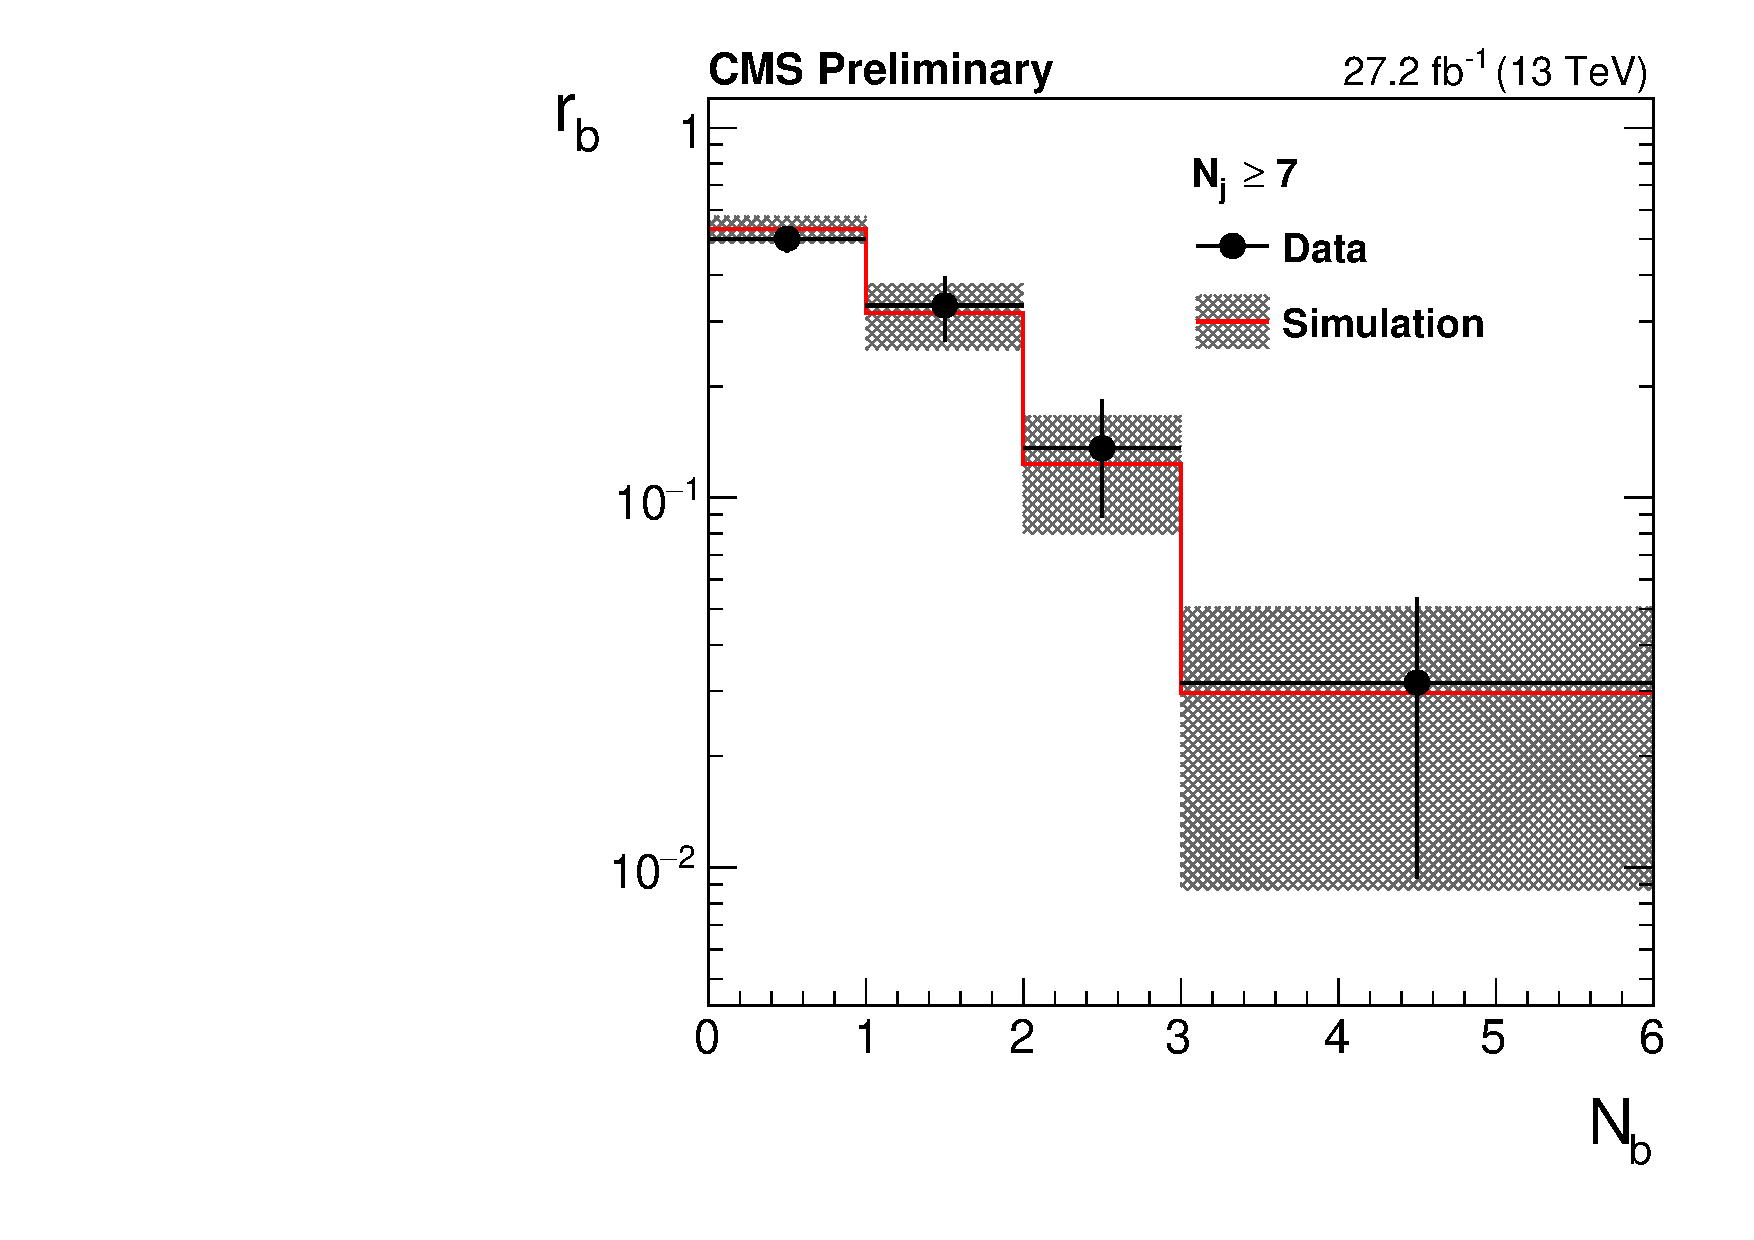
\includegraphics[width=0.45\textwidth]{backgrounds/figs/r_hat_HT250toInf_j7toInf_b0toInf}
	\caption{The values of \rb as measured in data in different \nj regions, compared to simulation. The uncertainties include both the statistical error and the systematic sources as listed in table \ref{tbl:fjrbSyst}}
	\label{fig:rb}
\end{figure}
\begin{table}
	\centering
	\caption{Relative uncertainty of \fj and \rb associated with the assumed invariance with respect to \mttwo and \dphi (and \HT for \rb).}
	 \begin{tabular}{c|ccc|cccc}
      \hline\hline
Observable    & $f_{23}$ & $f_{46}$ & $f_{7^+}$ & $ r_{0}$ & $ r_{1}$ & $ r_{2}$ & $ r_{3+}$\\\hline
Syst. Error   &  25\%   &   7\%   &   20\%   &    8\%       &     20\%     &     35\%    &    70\%      \\ 
\hline\hline
       \end{tabular}
	\label{tbl:fjrbSyst}
\end{table}


\subsection{Monojet Signal Region Prediction}
\label{subsec:qcdMonojet}
The multijet background in control regions with a single jet cannot be estimated using the \dphi technique since \MET is usually very similar to the \HT in these events and typically anti-aligned with the jet. As outlined in section \ref{subsec:multijetCR}, a separate control region is devised which instead selects dijet events that are orthogonal to the multijet signal regions because of an inverted \dphilong cut (and orthogonal to the the monojet SR with the presence of multiple jets). 

The sub-leading jet momentum for in this CR can be seen in figure \ref{fig:subleadingJetPt}. Because jets with \pt below 30\GeV are not considered, monojet events can be classified as those with $p_{\mathrm{T}}^{\mathrm{jet2}} < 30\GeV$, and the CR is used to extrapolate into the regime where $p_{\mathrm{T}}^{\mathrm{jet2}}$ is small. With decreasing $p_{\mathrm{T}}^{\mathrm{jet2}}$, events appear more imbalanced and approximate the topology of a true monojet event, as depicted in figure \ref{fig:monojetCartoon}.
\begin{figure}
	\centering
	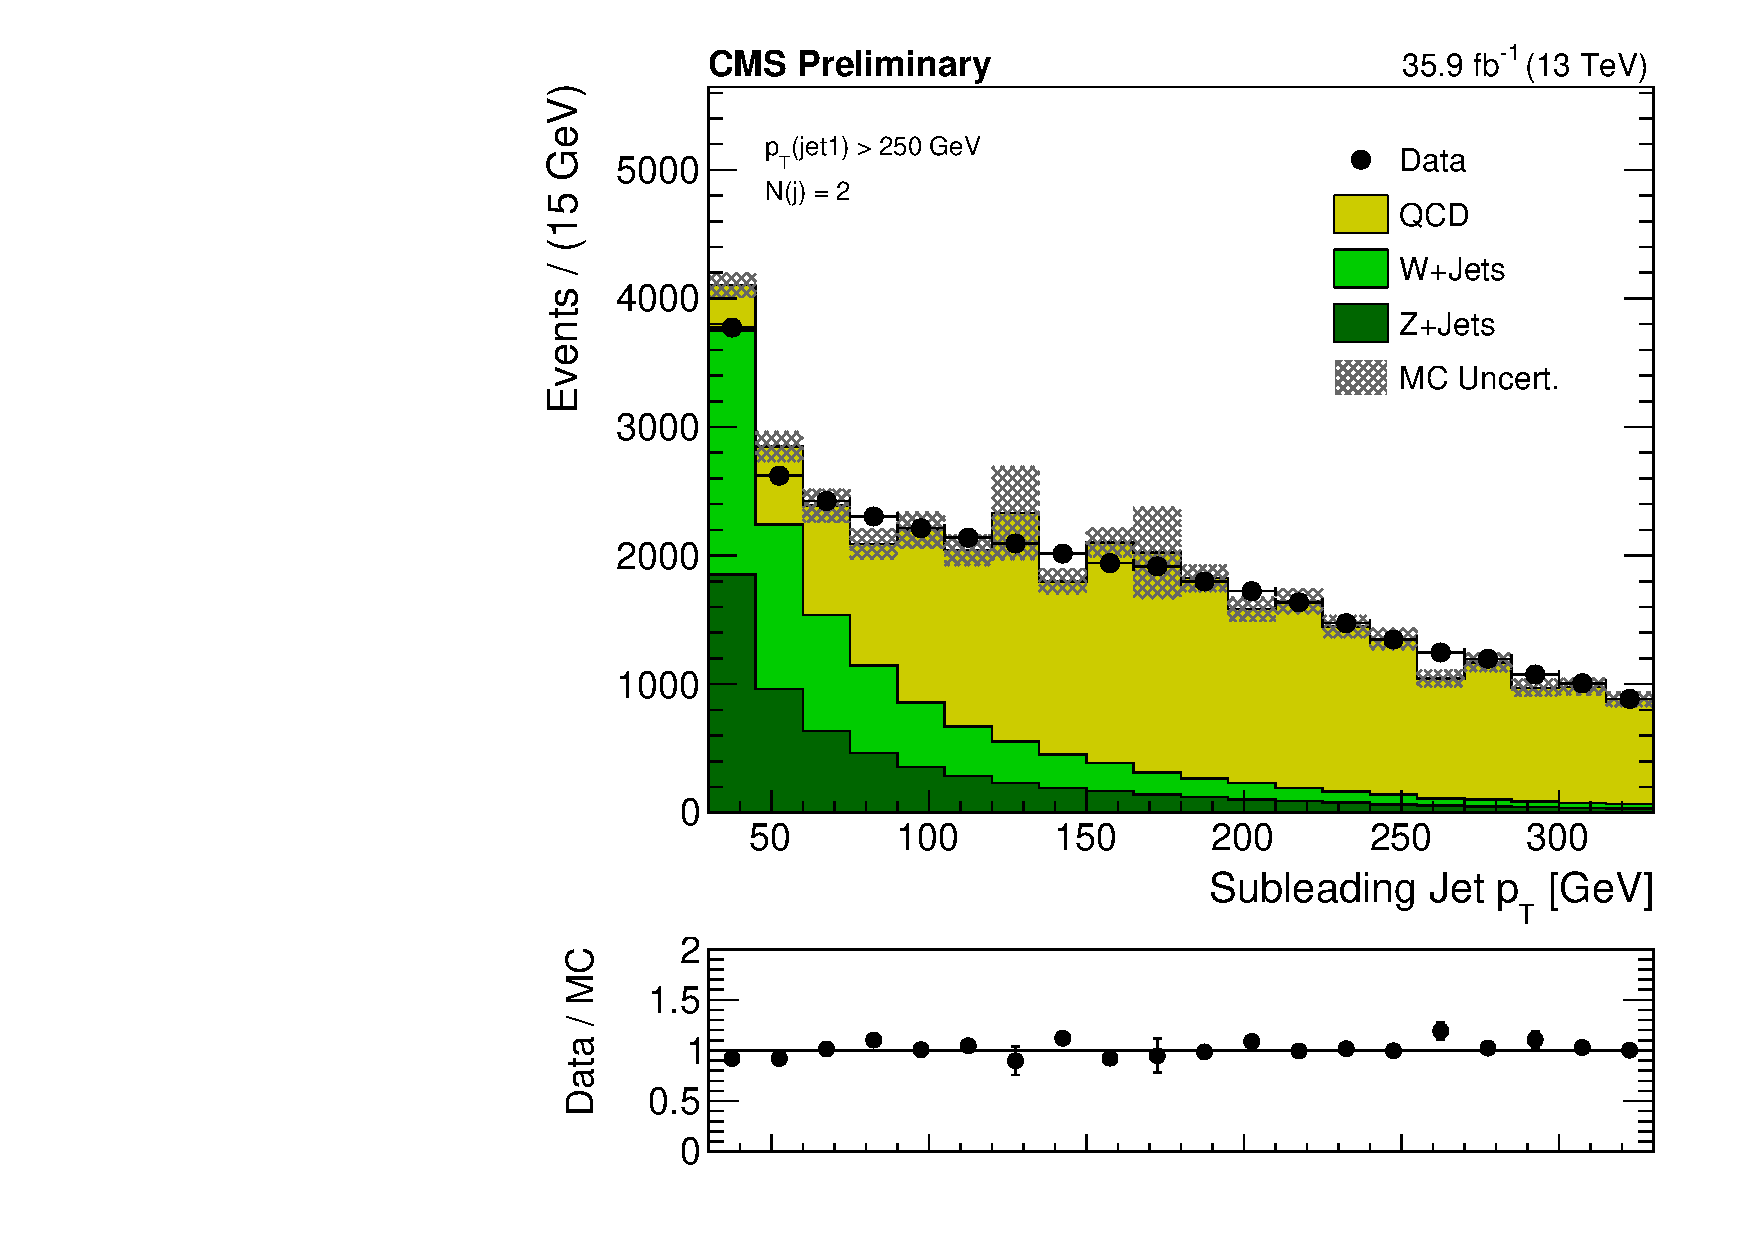
\includegraphics[width=0.45\textwidth]{backgrounds/figs/jet2_pt_35p9ifb}
	\caption{The transverse momentum of the sub-leading jet for dijet events in the monojet QCD background control region. The total yield of the simulation is normalized to the overall yield in data.}
	\label{fig:subleadingJetPt}
\end{figure}
\begin{figure}
	\centering
	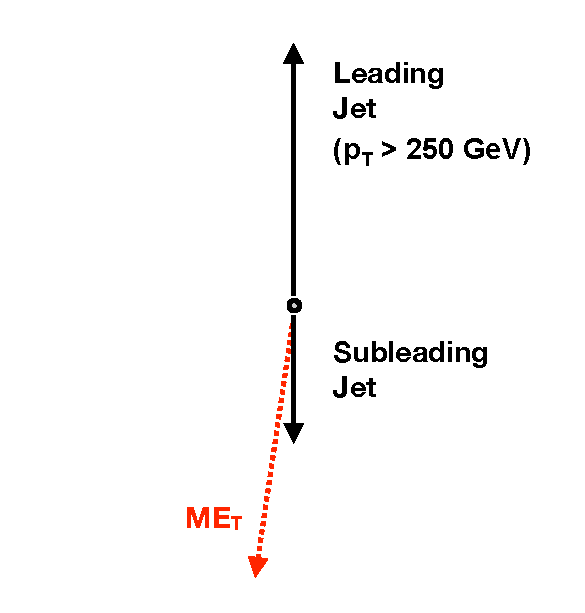
\includegraphics[width=0.45\textwidth]{backgrounds/figs/dijet_cartoon_Moriond2017}
	\caption{An illustration of ``unbalanced'' dijet events. As the momentum of the sub-leading jet decreases, \MET is more anti-aligned with the primary jet and approaches the topology of a monojet event.}
	\label{fig:monojetCartoon}
\end{figure}

The predicted yield of multijet background in a monojet $p_{\mathrm{T}}^{\mathrm{jet1}}$ bin is determined according to equation \ref{eq:monojetEstimate}, where $f_{\mathrm{QCD}}$ is the fraction of QCD events as measured in the region with $30 < p_{\mathrm{T}}^{\mathrm{jet2}} < 60 \GeV$ and $N_{\mathrm{data}}$ is the yield in data of dijet events with $30 < p_{\mathrm{T}}^{\mathrm{jet2}} < 60 \GeV$. Assuming $N_{\mathrm{data}}(0-30) < N_{\mathrm{data}}(30-60)$, this estimate provides an upper bound on the total multijet background contribution in each monojet CR. A systematic uncertainty of 50\% on the QCD fraction $f_{\mathrm{QCD}}$ is assigned as a conservative estimate.
\begin{equation}
	N_{\mathrm{QCD}}(p_{\mathrm{T}}^{\mathrm{jet1}}) = N_{\mathrm{data}}(30-60,p_{\mathrm{T}}^{\mathrm{jet1}}) \cdot f_{\mathrm{QCD}}(30-60,p_{\mathrm{T}}^{\mathrm{jet1}})
	\label{eq:monojetEstimate}
\end{equation}

% --------------------------------------------------------------------------- %
% --------------------------------------------------------------------------- %

% --------------------------------------------------------------------------- %
% --------------------------------------------------------------------------- %
\section{Lost Lepton Estimate}
\label{sec:lostlep}

The lost lepton background is predicted by taking the yield of single lepton events in similar kinematic regions, measuring the ratio of events where the lepton is lost to those where it is found, and extrapolating into the lost lepton regime. The control region for the lost lepton estimate is described in detail in section \ref{subsec:leptonCR}, and is comprised of events in data with the same signal triggers and preselection, with the exception of an inverted lepton veto and an additional requirement on lepton $M_{\mathrm{T}}$ (to reduce signal contamination). 

\subsection{Background Prediction}
\label{subsec:lostlepPrediction}

The estimate in a given signal region is obtained from a control region using transfer factors as described in equation \ref{eq:lostlepEstimate}, where $N_{\mathrm{1L}}^{\mathrm{CR}}$ is the number of events in the corresponding CR, $R_{\mathrm{MC}}^{0l/1l}$ is the ratio of zero-lepton to one-lepton events derived from simulation, and $k(\mttwomath)$ is the transfer factor into bins of \mttwo in a given topological region. The ratio $R_{\mathrm{MC}}^{0l/1l}$ is measured in Monte Carlo after normalizing the yield to data in each CR and correcting for differences in lepton efficiency between data and simulation, and also factors in lepton acceptance, efficiency of reconstruction and identification, as well as contributions from W bosons decaying through $\tau$ leptons to a hadronic final state. The \mttwo transfer factor $k(\mttwomath)$ is taken from data where statistics permit, and uses information from simulation to project events into bins of \mttwo in the low-statistics regime.
\begin{equation}
	N_{\mathrm{LL}}^{\mathrm{SR}}(\HT,N_\mathrm{j},N_\mathrm{b},\mttwomath) = N_{\mathrm{1L}}^{\mathrm{CR}}(\HT,N_\mathrm{j},N_\mathrm{b},\mttwomath) \cdot R_{\mathrm{MC}}^{0l/1l}(\HT,N_\mathrm{j},N_\mathrm{b},\mttwomath) \cdot k(\mttwomath)
	\label{eq:lostlepEstimate}
\end{equation}

To reduce the dependence of the estimate on the \mttwo shape modeling in simulation, the transfer factor $k(\mttwomath)$ uses a combination of data and simulation information. In each topological region, the greatest \mttwo bin is iteratively combined with the next-greatest bin until the total expected SM background yield in simulation is at least 50 events. These combined bins together form the CR for a range of \mttwo values, where the fraction of events falling in a particular \mttwo bin, $k(\mttwomath)$, is determined from simulation. In all the other \mttwo bins in the topological region, statistics are sufficient for a direct measurement in data and $k(\mttwomath)=1$. The extrapolation point for each topological region can be found in table \ref{tbl:lostlepHybridPoint}. The shape modeling in simulation is verified in data by selecting an inclusive sample enriched in either W boson or \ttbar production (using the number of b-tags in the event), and predicting the \mttwo distribution using simulation after normalizing simulation yield to data and summing all the control regions together, as seen in figure \ref{fig:lostlepHybrid}.
\begin{table}
	\centering
	\begin{tabular}[]{l c r}
		\fm{Table of lostlep hybrid extrapolation points} 
	\end{tabular}
	\caption{The last \mttwo bin and the \mttwo extrapolation point for each topological region, beyond which shape data from simulation is used to extrapolate the lost lepton estimate into \mttwo bins.}
	\label{tbl:lostlepHybridPoint}
\end{table}
\begin{figure}
	\centering
	
\includegraphics[width=0.45\textwidth]{figs/placeholder}
	
\includegraphics[width=0.45\textwidth]{figs/placeholder}
	\caption{The \mttwo shape in data and simulation using the single lepton CR selection, for events with zero b-tagged jets (left) or at least one b-tagged jet (right). The simulation is normalized to data in each topological region before summing to create the inclusive region. The hatched bands in each upper plot show the MC statistical uncertainty, while the shaded bands in each lower plot represent the systematic shape uncertainty.}
	\label{fig:lostlepHybrid}
\end{figure}

\subsection{Systematic Uncertainties}
\label{subsec:lostlepSyst}

Several sources of uncertainty are assessed for the lost lepton estimate, including those associated with the topological transfer factor and the \mttwo shape modeling in simulation. The full list of systematic uncertainties is as follows:
\begin{itemize}
	\item {\it Control region statistical error:} the Poisson error on the number of observed events in data is taken as a correlated uncertainty in each signal region using the same control region. The error is uncorrelated amongst \mttwo bins, except in regions sharing merged \mttwo bins for the estimate.
	\item {\it Monte Carlo statistical error:} where the simulation is used to compute the transfer factor (and in some cases, the \mttwo shape), the MC statistical uncertainty ranges from 1-50\%, taken as uncorrelated amongst all bins.
	\item {\it Electron and muon selection efficiency:} the reconstruction and identification efficiency of electrons and muons is computed using a procedure known as {\it tag and probe}, where leptons from \Zll decays are used to evaluate the lepton id efficiencies as a function of lepton \pt and $\eta$ and lepton isolation efficiencies as a function of \pt and nearby activity. The scale factors applied to simulation to compensate for such effects approach unity with uncertainties on the order of a few percent, and are correlated across all bins. The maximum effect of this uncertainty is up to 7\% in some signal regions.
	\item {\it Tau selection efficiency:} the efficiency for hadronically decaying taus is classified according to the number of charged particles in the $\tau$ decay, whether a {\it 1-prong} tau leaving a single charged track, or a {\it 3-prong} tau leaving three charged tracks in the final state. This efficiency is measured in simulation by measuring the isolation efficiency as a function of candidate \pt for electrons, muons, and taus in various decay modes. Based on half the difference in efficiency between 1-prong taus and muons, an uncertainty of 10\% is taken for 1-prong taus which also covers and differences in veto efficiency as a function of the primary kinematic variables. For 3-prong taus, the PF hadron veto is very inefficient since most fail the isolation requirement (the typical selection efficiency is 8\%), and a 100\% relative uncertainty is taken to cover any differences as a function of kinematics. These uncertainties are correlated amongst all bins.
	\item {\it \Mt cut efficiency:} the use of simulation to compute the CR-to-SR transfer factor also relies on the satisfactory modeling of the \Mt cut in Monte Carlo. A sample of \Zll events is selected in data with one of the leptons ``deleted'' from the event to mimic a leptonic W boson decay, and compared with simulation. Based on data-MC agreement, a correlated error of 3\% is taken across all bins.
	\item {\it b-tagging efficiency:} the effect of varying the b-tag scale factor efficiency is calculated in each bin, and taken as a correlated error amongst all bins. The maximum effect of this variation is about 4\% in some bins.
	\item {\it Jet energy corrections:} by varying the jet energy scales across all bins, a maximum deviation of about 5\% is observed in regions with sufficient statistics, and a correlated error of 5\% is taken across al bins.
	\item {\it MC renormalization and factorization scales:} the overall effect of varying the simulation renormalization and factorization scales of the underlying physics processes (and subsequent effect on event kinematics) are computed separately in each bin. Taken as correlated across all bins, they are typically on the order of a few percent but range up to 10\% in some regions.
	\item {\it \mttwo shape uncertainty:} in regions where the simulation is used to model the \mttwo distribution, additional variations of the renormalization and factorization scales, parton distribution functions, b-tagging scale factor uncertainties, and jet energy scale uncertainties are performed to measure their effect on the \mttwo shape modeling. The most significant impact is seen in the highest \mttwo bins from theoretical uncertainties ($\sim$15\%), and up to 40\% in low statistics bins due to jet energy scale variations. With this in mind, the shape uncertainty (in regions where MC \mttwo shape modeling is used) is assigned as a linear morphing of the \mttwo shape starting in the first bin from which MC extrapolation is used, growing to 40\% in the final bin. The shape morphing in every distinct topological region is taken as an uncorrelated error.
\end{itemize}


\subsection{Signal Contamination}
\label{subsec:signalContamination}

Nearly every control region in this analysis (including those for multijet and invisible Z backgrounds) is not only orthogonal to the signal region selection, but also crafted such that any potential BSM signal contribution to any CR is negligible and will not bias the background estimate. However, certain SUSY simplified models yield final states with prompt lepton decays --- in some cases kinematically similar to SM \ttbar decays --- which may be non-negligible in the lost lepton CR. To account for this effect when calculating limits on such models (described in detail in section ref{sec:interpretations}), the amount by which the lost lepton background is overestimated is modeled as a loss in signal efficiency. The modified signal yield $N_{\mathrm{sig}}^{SR\prime}$ is defined in equation \ref{eq:signalContamination}, where $N_{\mathrm{sig}}^{SR}$ and $N_{\mathrm{sig}}^{CR}$ represent the simulated signal yield in the signal and control regions respectively, and $TF$ the total transfer factor used in the lost lepton estimate for a given signal region. 
\begin{equation}
	N_{\mathrm{sig}}^{SR\prime} = N_{\mathrm{sig}}^{SR} - TF \cdot N_{\mathrm{sig}}^{CR}
	\label{eq:signalContamination}
\end{equation}
The correction is most significant for simplified models with stop decays, where the stop-neutralino mass splitting is close to the SM top quark mass. In such cases, the signal contamination is maximally 5\% of the expected background yields in each CR for mass points near the expected exclusion limits at high mass.


% --------------------------------------------------------------------------- %
% --------------------------------------------------------------------------- %

% --------------------------------------------------------------------------- %
% --------------------------------------------------------------------------- %
\section{Invisible Z Estimate}
\label{sec:zinv}

The invisible Z background is the dominant SM contribution in many signal regions due to the ``irreducible'' nature of the underlying physics. Because the primary interaction produces a massive particle decaying to an invisible final state (\znunu) recoiling against hadronic activity, the signature is fundamentally similar to that of the BSM physics the search is designed to target and difficult to reduce by conventional cuts removing SM background contributions. A robust method leveraging the well-understood Drell-Yan process (\zll) --- kinematically similar to the invisible Z background --- is used to predict the expected SM contribution based on data while minimizing the reliance on Monte Carlo modeling of the kinematics.

\subsection{Background Prediction}
\label{subsec:zinvPrediction}
The invisible Z background is estimated using dilepton events selected in data. The control region consists of events selected with dilepton triggers, with addition requirements that the leptons are of the same flavor and opposite sign. The momentum of the leading and trailing lepton must also be at least 100\GeV and 30\GeV, respectively, and the invariant mass of the lepton system \mll must be withing 20\GeV of the Z boson mass. The individual CRs are then constructed by removing the dilepton system from the event and applying the baseline preselection requirements as for the signal regions. A detailed description of the CR can be found in section \ref{subsec:zllCR}.

The invisible Z prediction is computed as described by equation \ref{eq:zinvEstimate}, where $N_{\ell\ell}^{\mathrm{CR(SF)}}$ is the number of events in the dilepton same-flavor (SF) region, $N_{\ell\ell}^{\mathrm{CR(OF)}}$ the number of events in the dilepton opposite-flavor (OF) region, $R^{\mathrm{SF/OF}}$ the SF-OF transfer factor, $R_{\mathrm{MC}}^{\znunu / \zll}$ the transfer factor from \zll to \znunu events, and $k(\mttwomath)$ the transfer factor into bins of \mttwo. Each factor is explained in detail below. 
\begin{align}
		N_{\znunu}^{\mathrm{SR}}(\HT,N_\mathrm{j},N_\mathrm{b},\mttwomath) =& \left[ N_{\ell\ell}^{\mathrm{CR(SF)}}(\HT,N_\mathrm{j},N_\mathrm{b}) - N_{\ell\ell}^{\mathrm{CR(OF)}}(\HT,N_\mathrm{j},N_\mathrm{b}) \cdot R^{\mathrm{SF/OF}} \right] \nonumber \\
		& \times R_{\mathrm{MC}}^{\znunu / \zll}(\HT,N_\mathrm{j},N_\mathrm{b}) \cdot k(\mttwomath)
	\label{eq:zinvEstimate}
\end{align}

The second term in equation \ref{eq:zinvEstimate}, $N_{\ell\ell}^{\mathrm{CR(OF)}}\cdot R^{\mathrm{SF/OF}}$, is a correction factor applied to the control region yield to correct for the contribution from processes producing SF and OF event, or {\it flavor-symmetric processes} (such as \ttbar). To compensate for this contribution, a separate control region enriched in \ttbar events is selected from data by using the same selections as the invisible Z CR, except for an inverted selection on the dilepton \pt and \mll requirements. The ratio of \ttbar events is then measured directly from data by counting the yield of SF ($ee$ or $\mu\mu$) and OF ($e\mu$ or $\mu e$) events in this CR. The ratio $R^{\mathrm{SF/OF}}$ is expected to be close to unity based on the underlying physics process, but due to varying acceptance and efficiency effects for different flavor leptons is measured as $R^{\mathrm{SF/OF}} = 1.13 \pm 0.15$, and is stable with respect to event kinematics as shown in figure \ref{fig:rsfof}. The Drell-Yan yield in each control region, as well as the SF yield, OF yield, and transfer factors can be found in tables \ref{tbl:zinvCRs1} and \ref{tbl:zinvCRs2}.
\begin{figure}
	\centering
	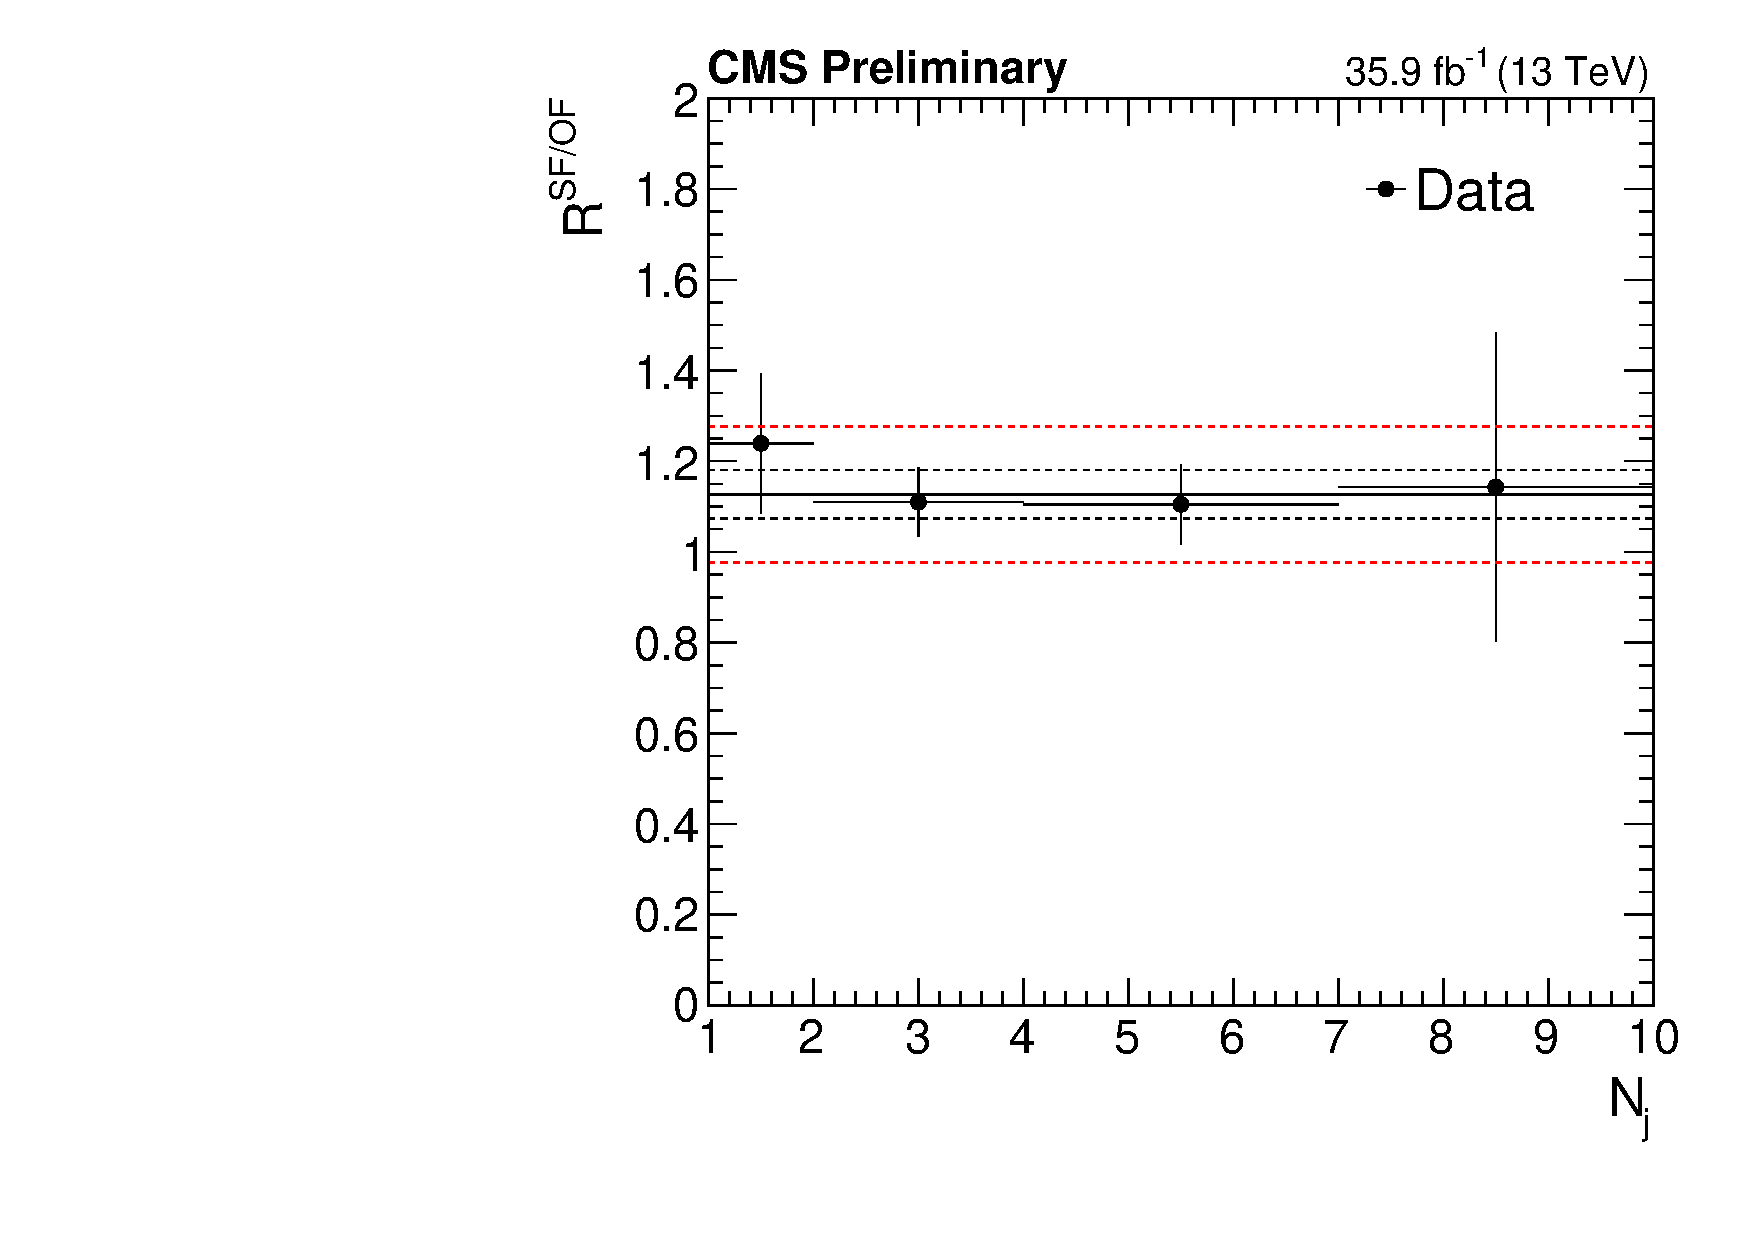
\includegraphics[width=0.45\textwidth]{backgrounds/figs/RSFOF_nj}
	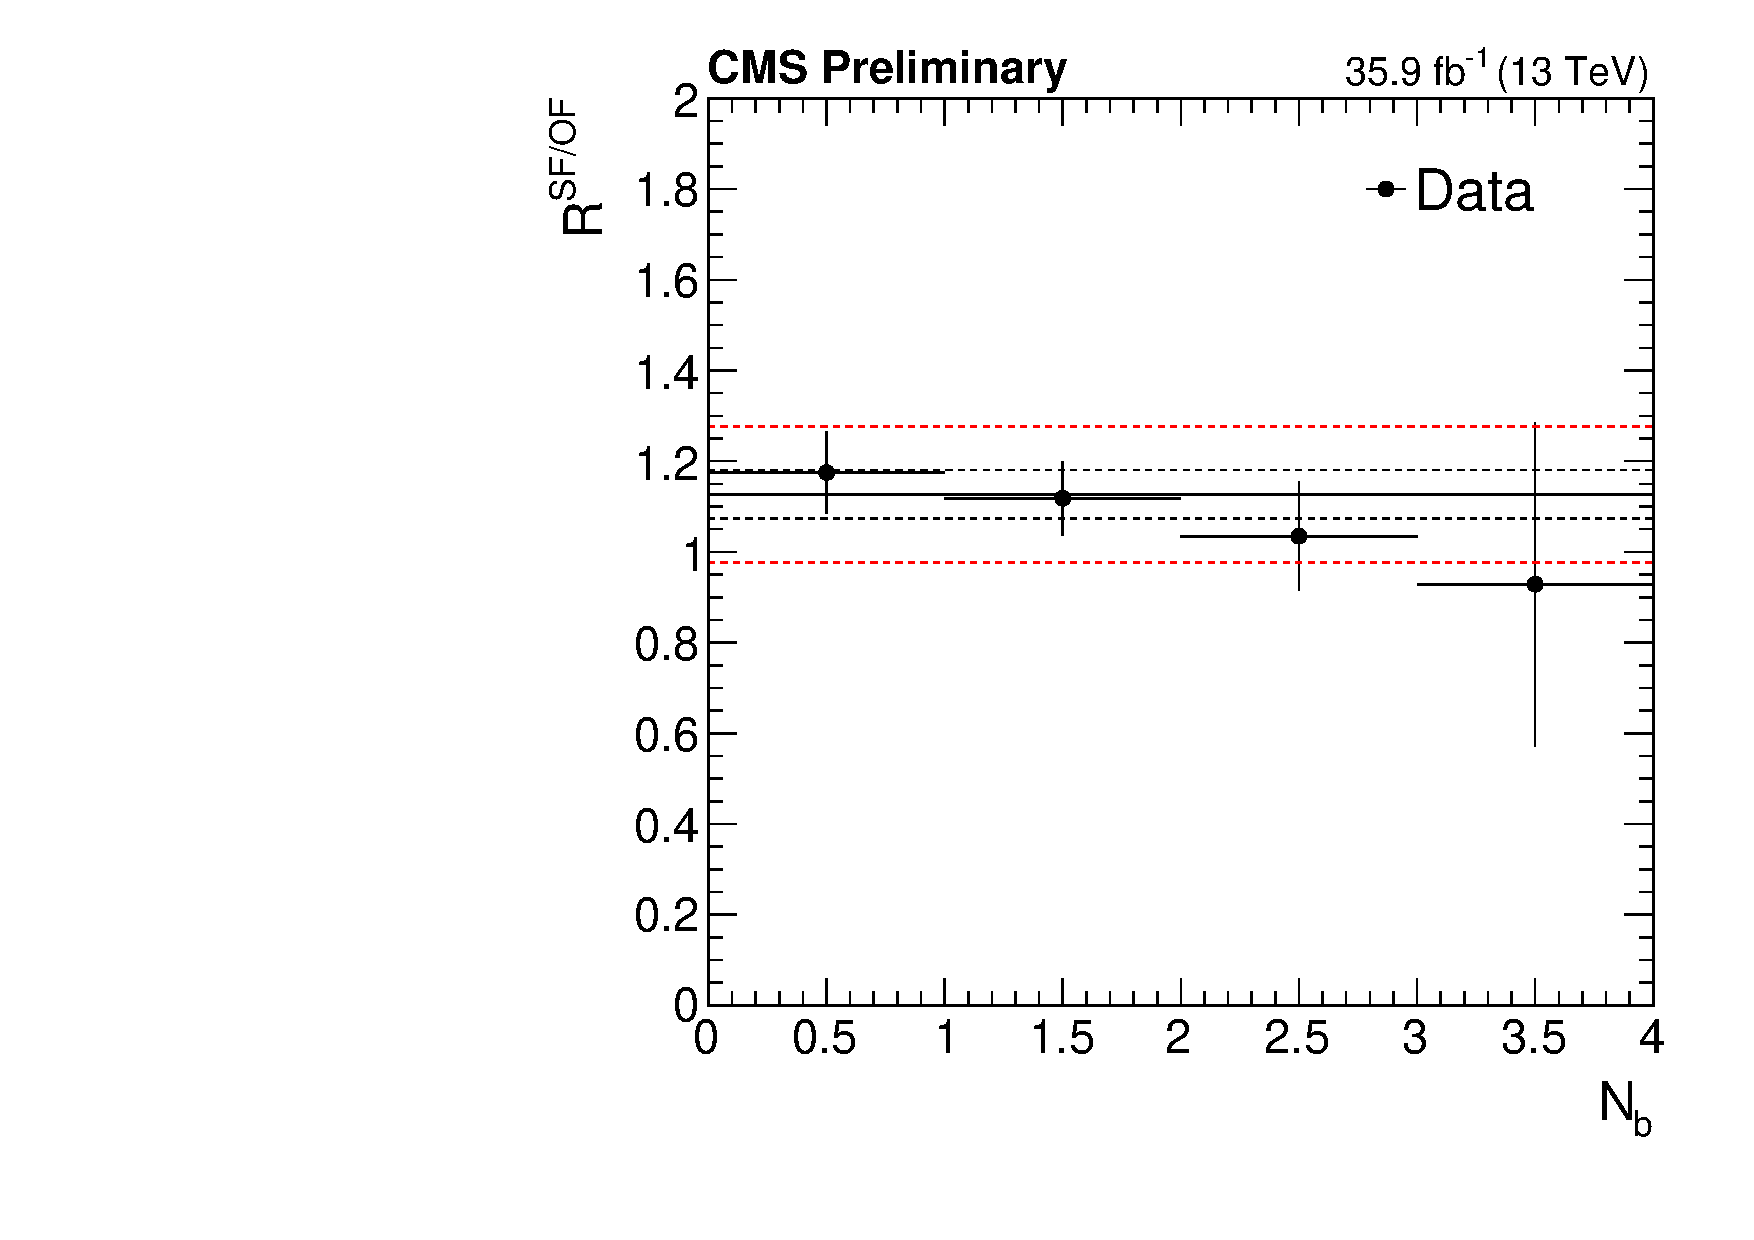
\includegraphics[width=0.45\textwidth]{backgrounds/figs/RSFOF_nb}
	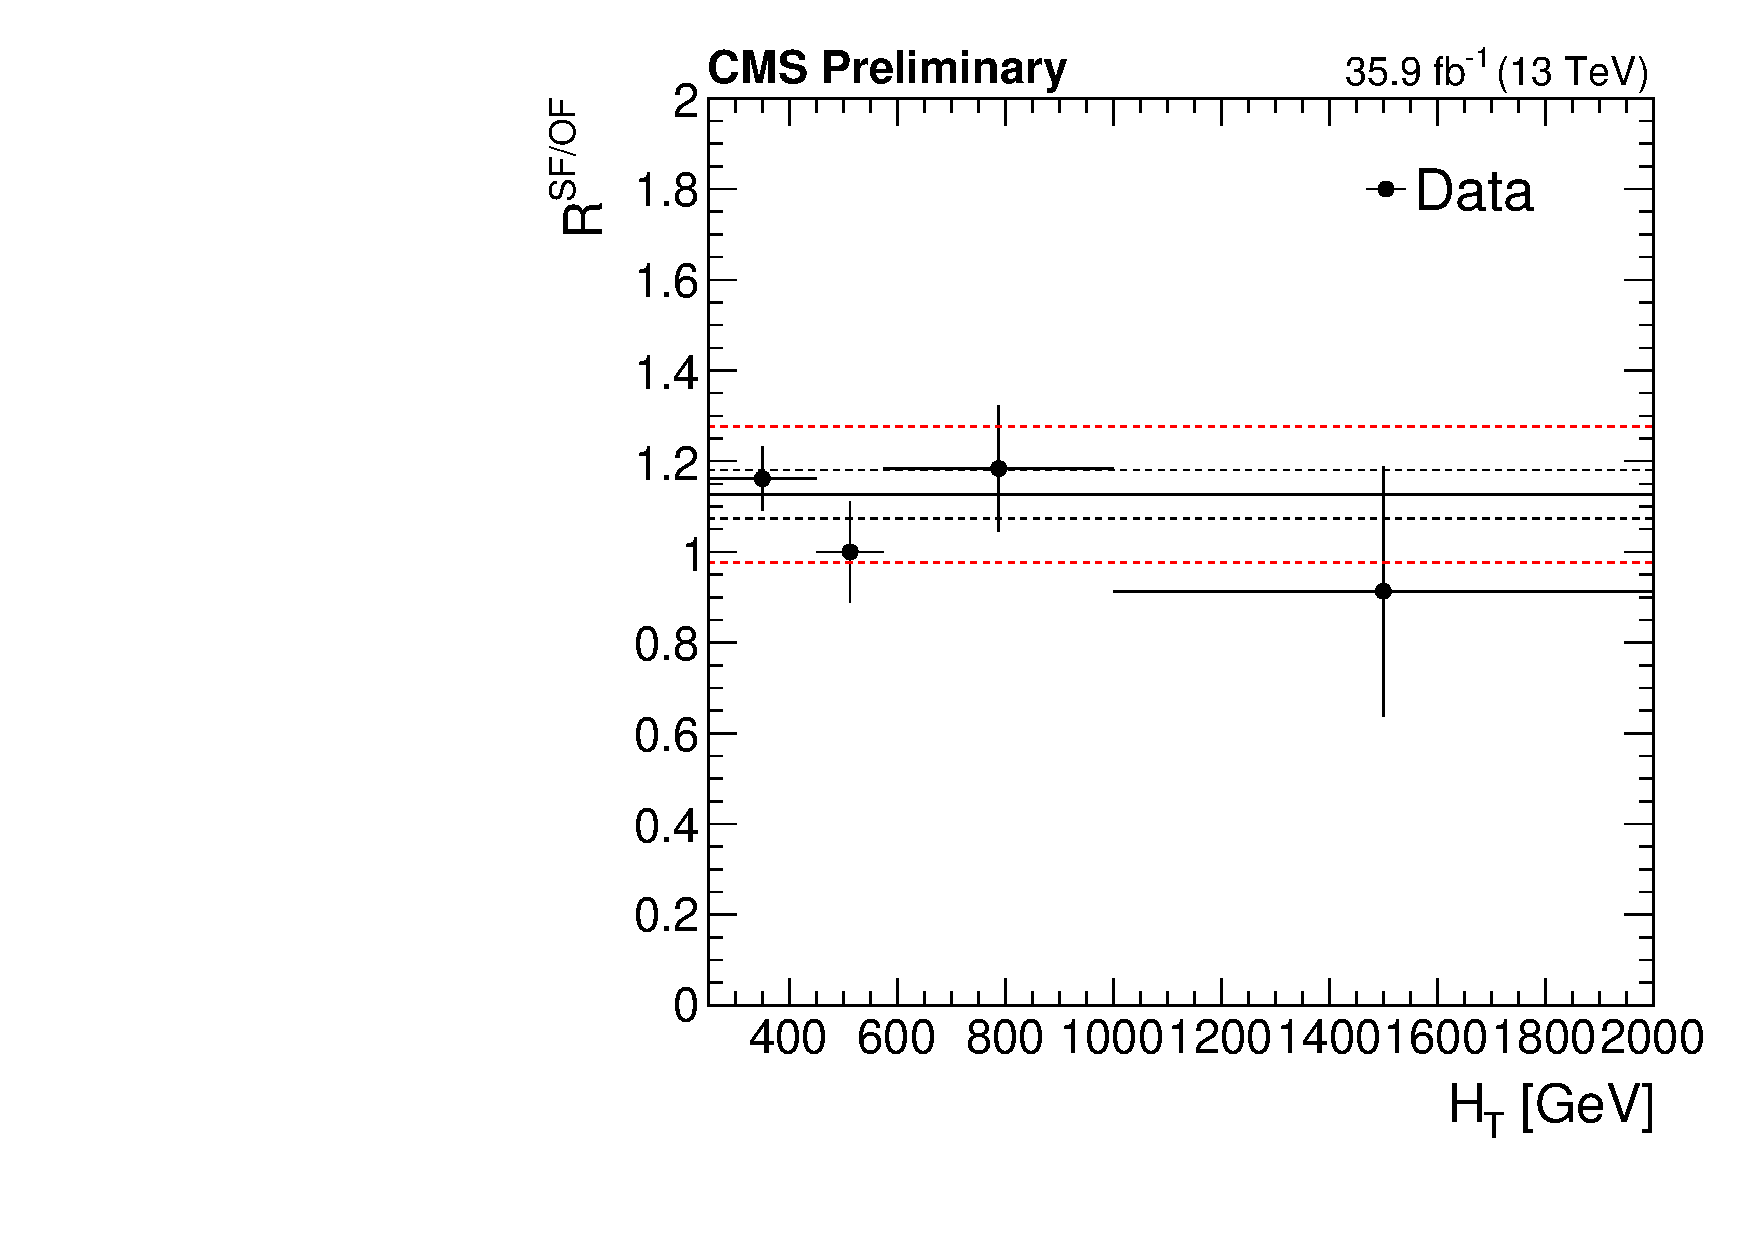
\includegraphics[width=0.45\textwidth]{backgrounds/figs/RSFOF_ht}
	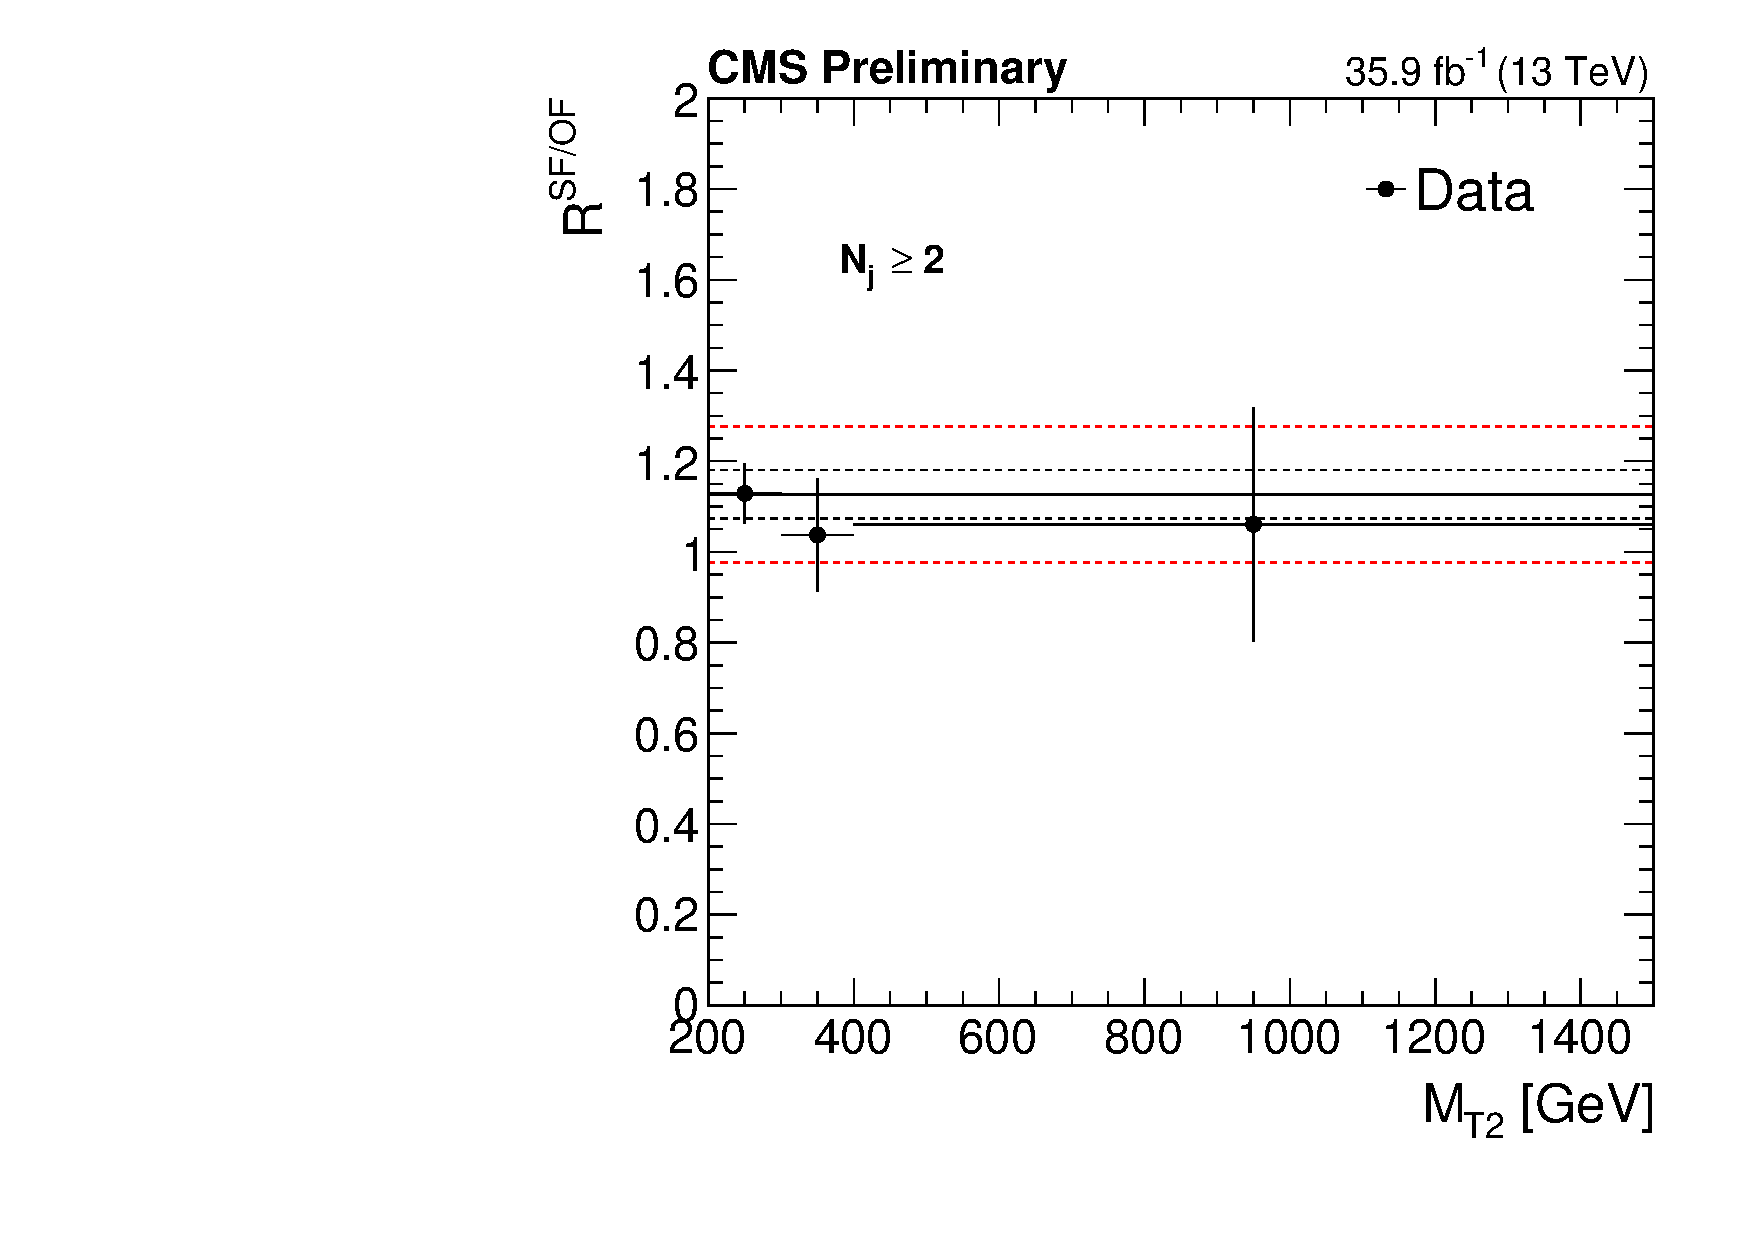
\includegraphics[width=0.45\textwidth]{backgrounds/figs/RSFOF_mt2}
	\renewcommand{\baselinestretch}{1.0}
	\caption[The ratio of same-flavor to opposite-flavor events in a \ttbar enriched control region, as a function of \nj (top left), \nb (top right), \HT (bottom left), and \mttwo (bottom left).]{The ratio of same-flavor to opposite-flavor events in a \ttbar enriched control region, as a function of \nj (top left), \nb (top right), \HT (bottom left), and \mttwo (bottom left). The solid black line corresponds to a constant value of $1.13 \pm 0.15$, while the dashed black lines correspond to the statistical uncertainty and the dashed red lines the total systematic uncertainty.}
	\label{fig:rsfof}
\end{figure}
\begin{table}
	\centering
	\renewcommand{\baselinestretch}{1.0}
	\caption[The control region predicted Drell-Yan (DY) yield, SF yield, OF yield, purity (the rfraction of \zll events), and ratio $R_{\mathrm{MC}}^{\znunu / \zll}$ for the very low, low, and medium \HT topological regions.]{The control region predicted Drell-Yan (DY) yield, SF yield, OF yield, purity (the rfraction of \zll events), and ratio $R_{\mathrm{MC}}^{\znunu / \zll}$ for the very low, low, and medium \HT topological regions. Note that the 7+ jet regions with b-tags (marked with an asterisk) share the same CR, and the fraction of events with different numbers of b-tags is folded into the ratio.}
	\small
	\renewcommand{\arraystretch}{1.0}
	\begin{tabular}{c|c|c|c|c|c|c|c}
\hline \hline
\multicolumn{8}{c}{Invisible Z} \\
\hline
\multicolumn{3}{c|}{Region} & DY Yield & SF Yield & OF Yield & Purity & Ratio\\
$\text{H}_{T}$ [GeV] & $\text{N}_{j}$ & $\text{N}_{b}$ & & & &  \\
\hline
$[250,450]$ &2-3&0&8707.6&8749&37&0.995$\pm$0.001&5.61\\
$[250,450]$ &2-3&1&986.0&1005&17&0.981$\pm$0.004&5.47\\
$[250,450]$ &2-3&2&122.8&125&2&0.982$\pm$0.012&5.31\\
$[250,450]$ &4+&0&1124.5&1129&4&0.996$\pm$0.002&5.88\\
$[250,450]$ &4+&1&215.2&223&7&0.965$\pm$0.012&5.70\\
$[250,450]$ &4+&2&35.9&37&1&0.970$\pm$0.028&5.52\\
$[250,450]$ &2-3&3+&7.0&7&0&1.000$\pm$0.000&6.29\\
$[450,575]$ &2-3&0&1862.7&1875&11&0.993$\pm$0.002&5.08\\
$[450,575]$ &2-3&1&273.2&281&7&0.972$\pm$0.010&4.89\\
$[450,575]$ &2-3&2&19.8&22&2&0.898$\pm$0.064&4.75\\
$[450,575]$ &4-6&0&650.9&661&9&0.985$\pm$0.005&5.49\\
$[450,575]$ &4-6&1&143.4&149&5&0.962$\pm$0.016&5.58\\
$[450,575]$ &4-6&2&27.6&31&3&0.892$\pm$0.056&5.21\\
$[450,575]$ &7+&0&7.0&7&0&1.000$\pm$0.000&5.56\\
$[450,575]$ &7+&1&4.0&4&0&1.000$\pm$0.000&5.18$^{(*)}$\\
$[450,575]$ &7+&2&4.0&4&0&1.000$\pm$0.000&1.87$^{(*)}$\\
$[450,575]$ &2-6&3+&7.0&7&0&1.000$\pm$0.000&5.78\\
$[450,575]$ &7+&3+&4.0&4&0&1.000$\pm$0.000&0.48$^{(*)}$\\
$[575,1000]$ &2-3&0&1347.0&1356&8&0.993$\pm$0.002&4.76\\
$[575,1000]$ &2-3&1&157.3&164&6&0.959$\pm$0.015&4.55\\
$[575,1000]$ &2-3&2&25.8&28&2&0.920$\pm$0.051&4.68\\
$[575,1000]$ &4-6&0&812.4&818&5&0.993$\pm$0.003&5.16\\
$[575,1000]$ &4-6&1&180.0&189&8&0.953$\pm$0.015&5.09\\
$[575,1000]$ &4-6&2&26.3&33&6&0.796$\pm$0.070&5.29\\
$[575,1000]$ &7+&0&32.9&34&1&0.967$\pm$0.031&5.84\\
$[575,1000]$ &7+&1&15.6&19&3&0.823$\pm$0.088&4.41$^{(*)}$\\
$[575,1000]$ &7+&2&15.6&19&3&0.823$\pm$0.088&1.10$^{(*)}$\\
$[575,1000]$ &2-6&3+&5.8&8&2&0.720$\pm$0.159&5.82\\
$[575,1000]$ &7+&3+&15.6&19&3&0.823$\pm$0.088&0.22$^{(*)}$\\
\hline \hline
	\end{tabular}
	\label{tbl:zinvCRs1}
\end{table}

\begin{table}
	\centering
	\renewcommand{\baselinestretch}{1.0}
	\caption[The control region predicted Drell-Yan (DY) yield, SF yield, OF yield, purity (the rfraction of \zll events), and ratio $R_{\mathrm{MC}}^{\znunu / \zll}$ for the high and extreme \HT topological regions.]{The control region predicted Drell-Yan (DY) yield, SF yield, OF yield, purity (the rfraction of \zll events), and ratio $R_{\mathrm{MC}}^{\znunu / \zll}$ for the high and extreme \HT topological regions. Note that the 7+ jet regions with b-tags (marked with an asterisk) share the same CR, and the fraction of events with different numbers of b-tags is folded into the ratio.}
	\small
	\renewcommand{\arraystretch}{1.0}
	\begin{tabular}{c|c|c|c|c|c|c|c}
\hline \hline
\multicolumn{8}{c}{Invisible Z} \\
\hline
\multicolumn{3}{c|}{Region} & DY Yield & SF Yield & OF Yield & Purity & Ratio\\
$\text{H}_{T}$ [GeV] & $\text{N}_{j}$ & $\text{N}_{b}$ & & & &  \\
\hline
$[1000,1500]$ &2-3&0&129.0&129&0&1.000$\pm$0.000&4.76\\
$[1000,1500]$ &2-3&1&25.9&27&1&0.959$\pm$0.038&4.63\\
$[1000,1500]$ &2-3&2&1.9&3&1&0.627$\pm$0.279&4.73\\
$[1000,1500]$ &4-6&0&154.0&154&0&1.000$\pm$0.000&5.10\\
$[1000,1500]$ &4-6&1&42.0&42&0&1.000$\pm$0.000&4.97\\
$[1000,1500]$ &4-6&2&11.0&11&0&1.000$\pm$0.000&5.07\\
$[1000,1500]$ &7+&0&19.0&19&0&1.000$\pm$0.000&5.63\\
$[1000,1500]$ &7+&1&10.0&10&0&1.000$\pm$0.000&4.63$^{(*)}$\\
$[1000,1500]$ &7+&2&10.0&10&0&1.000$\pm$0.000&1.22$^{(*)}$\\
$[1000,1500]$ &2-6&3+&1.0&1&1&1.000$\pm$1.000&4.25\\
$[1000,1500]$ &7+&3+&10.0&10&0&1.000$\pm$0.000&0.20$^{(*)}$\\
$[1500,\infty]$ &2-3&0&29.0&29&0&1.000$\pm$0.000&5.00\\
$[1500,\infty]$ &2-3&1&8.0&8&0&1.000$\pm$0.000&4.66\\
$[1500,\infty]$ &4-6&0&28.9&30&1&0.963$\pm$0.035&5.09\\
$[1500,\infty]$ &4-6&1&14.0&14&0&1.000$\pm$0.000&5.25\\
$[1500,\infty]$ &4-6&2&2.9&4&1&0.720$\pm$0.224&4.80\\
$[1500,\infty]$ &7+&0&5.0&5&0&1.000$\pm$0.000&5.16\\
$[1500,\infty]$ &7+&1&1.9&3&1&0.627$\pm$0.279&3.97$^{(*)}$\\
$[1500,\infty]$ &7+&2&1.9&3&1&0.627$\pm$0.279&1.18$^{(*)}$\\
$[1500,\infty]$ &2-6&3+&1.0&1&0&1.000$\pm$0.000&6.27\\
$[1500,\infty]$ &7+&3+&1.9&3&1&0.627$\pm$0.279&0.18$^{(*)}$\\
\hline \hline
	\end{tabular}
	\label{tbl:zinvCRs2}
\end{table}

The ratio of invisible Z events to Drell-Yan events, $R_{\mathrm{MC}}^{\znunu / \zll}$, is measured in simulation for each CR. The ratio accounts for the branching fraction differences between \zll and \znunu decays, as well as differences in lepton acceptance and efficiency for dilepton pairs in the CR (including corrections for differences in lepton efficiency between data and simulation).

The transfer factor $k(\mttwomath)$ uses a combination of data and simulation information to reduce the dependence of the prediction on the \mttwo shape modeling in simulation. Based on simulation, the \mttwo shape in ever \HT region is independent of \nb. In addition, in the extreme \HT region $\HT > 1500\GeV$, the shape is also independent of \nj. Based on these findings, \mttwo shape templates are constructed for each \HT and \nj region (inclusive in \nb\footnote{The only exception is for regions with more than 2 b-tags (2j3b and 2-6j3b), where at least 3 jets are required so as to avoid biasing the \nj distribution when requiring more b-tags than jets.}), with one single template for the extreme \HT region (which is also inclusive in \nj). 

The \mttwo distribution, $k(\mttwomath)$, for each topological region is constructed from dilepton events in data where statistics allows, and \znunu simulation where statistics are sparse. In each template region, the greatest \mttwo bin is iteratively combined with the next-greatest bin until the total expected SM background yield in simulation is at least 50 events. For uncombined bins (where statistics in data is sufficient), the \mttwo shape is taken directly from dilepton data, corrected for the ratio $R_{\mathrm{MC}}^{\znunu / \zll}$. In the low-statistics combined regime, the \mttwo shape in \znunu simulation is used to determine the fraction of events in each \mttwo bin after normalizing the simulation yield to data in the combined bins. The extrapolation point after which the \mttwo shape is based on simulation in each signal region can be found in tables \ref{tbl:zinvHybridPoint1} and \ref{tbl:zinvHybridPoint2}.
\begin{table}
	\centering
	\renewcommand{\baselinestretch}{1.0}
	\caption[The \mttwo extrapolation point for the very low, low, and medium \HT topological regions, beyond which shape data from simulation is used to extrapolate the invisible Z estimate into \mttwo bins.]{The \mttwo extrapolation point for the very low, low, and medium \HT topological regions, beyond which shape data from simulation is used to extrapolate the invisible Z estimate into \mttwo bins. ``NA'' indicates regions where the simulation shape is not used at all since dilepton statistics in data are sufficiently large to perform the estimate bin-by-bin.}
	\small
	\renewcommand{\arraystretch}{1.0}
	\begin{tabular}{c|c|c|c}
\hline \hline
\multicolumn{4}{c}{Invisible Z} \\
\hline
\multicolumn{3}{c|}{Template Region} & Extrapolation Point\\
$\text{H}_{T}$ [GeV] & $\text{N}_{j}$ & $\text{N}_{b}$ & $\text{M}_{T2}$ [GeV]\\
\hline
$[250,450]$ &2-3&0& NA \\
$[250,450]$ &2-3&1& NA \\
$[250,450]$ &2-3&2& NA \\
$[250,450]$ &4+&0& 300 \\
$[250,450]$ &4+&1& 300 \\
$[250,450]$ &4+&2& 300 \\
$[250,450]$ &2+&3+& NA \\
$[450,575]$ &2-3&0& 400 \\
$[450,575]$ &2-3&1& 400 \\
$[450,575]$ &2-3&2& 400 \\
$[450,575]$ &4-6&0& 400 \\
$[450,575]$ &4-6&1& 400 \\
$[450,575]$ &4-6&2& 400 \\
$[450,575]$ &7+&0& 200 \\
$[450,575]$ &7+&1& 200 \\
$[450,575]$ &7+&2& 200 \\
$[450,575]$ &2-6&3+& NA \\
$[450,575]$ &7+&3+& 200 \\
$[575,1000]$ &2-3&0& 600 \\
$[575,1000]$ &2-3&1& 600 \\
$[575,1000]$ &2-3&2& 600 \\
$[575,1000]$ &4-6&0& 600 \\
$[575,1000]$ &4-6&1& 600 \\
$[575,1000]$ &4-6&2& 600 \\
$[575,1000]$ &7+&0& 200 \\
$[575,1000]$ &7+&1& 200 \\
$[575,1000]$ &7+&2& 200 \\
$[575,1000]$ &2-6&3+& NA \\
$[575,1000]$ &7+&3+& 200 \\
\hline \hline
	\end{tabular}
	\label{tbl:zinvHybridPoint1}
\end{table}

\begin{table}
	\centering
	\renewcommand{\baselinestretch}{1.0}
	\caption[The \mttwo extrapolation point for the high and extreme \HT topological regions, beyond which shape data from simulation is used to extrapolate the invisible Z estimate into \mttwo bins.]{The \mttwo extrapolation point for the high and extreme \HT topological regions, beyond which shape data from simulation is used to extrapolate the invisible Z estimate into \mttwo bins. ``NA'' indicates regions where the simulation shape is not used at all since dilepton statistics in data are sufficiently large to perform the estimate bin-by-bin.}
	\small
	\renewcommand{\arraystretch}{1.0}
	\begin{tabular}{c|c|c|c}
\hline \hline
\multicolumn{4}{c}{Invisible Z} \\
\hline
\multicolumn{3}{c|}{Template Region} & Extrapolation Point\\
$\text{H}_{T}$ [GeV] & $\text{N}_{j}$ & $\text{N}_{b}$ & $\text{M}_{T2}$ [GeV]\\
\hline

$[1000,1500]$ &2-3&0& 400 \\
$[1000,1500]$ &2-3&1& 400 \\
$[1000,1500]$ &2-3&2& 400 \\
$[1000,1500]$ &4-6&0& 400 \\
$[1000,1500]$ &4-6&1& 400 \\
$[1000,1500]$ &4-6&2& 400 \\
$[1000,1500]$ &7+&0& 200 \\
$[1000,1500]$ &7+&1& 200 \\
$[1000,1500]$ &7+&2& 200 \\
$[1000,1500]$ &2-6&3+& NA \\
$[1000,1500]$ &7+&3+& 200 \\
$[1500,\infty]$ &2-3&0& 400 \\
$[1500,\infty]$ &2-3&1& 400 \\
$[1500,\infty]$ &4-6&0& 400 \\
$[1500,\infty]$ &4-6&1& 400 \\
$[1500,\infty]$ &4-6&2& 400 \\
$[1500,\infty]$ &7+&0& 400 \\
$[1500,\infty]$ &7+&1& 400 \\
$[1500,\infty]$ &7+&2& 400 \\
$[1500,\infty]$ &2-6&3+& 400 \\
$[1500,\infty]$ &7+&3+& 400 \\
\hline \hline
	\end{tabular}
	\label{tbl:zinvHybridPoint2}
\end{table}

The accuracy of the \mttwo shape modeling in simulation is verified using other control samples enriched in $\gamma$, \wlnu, and \zll events in each \HT bin, as shown in figure \ref{fig:zinvMt2Shape}. The $\gamma$-enriched sample is selected using photon triggers and requiring $p_{\mathrm{T}}^{\gamma} > 180\GeV$, with corrections applied for multijet background contributions and the ratio of \mttwo distributions for photon to Z boson events, $R_{\mathrm{MC}}^{\mathrm{Z}/\gamma}$. The W and Z boson samples are selected in data using leptonic triggers, corrected to compensate for the contribution from top quark production, as well as the ratio of \mttwo distributions, $R_{\mathrm{MC}}^{\mathrm{Z}/W}$ and $R_{\mathrm{MC}}^{\znunu/\zll}$ respectively.
\begin{figure}
	\centering
	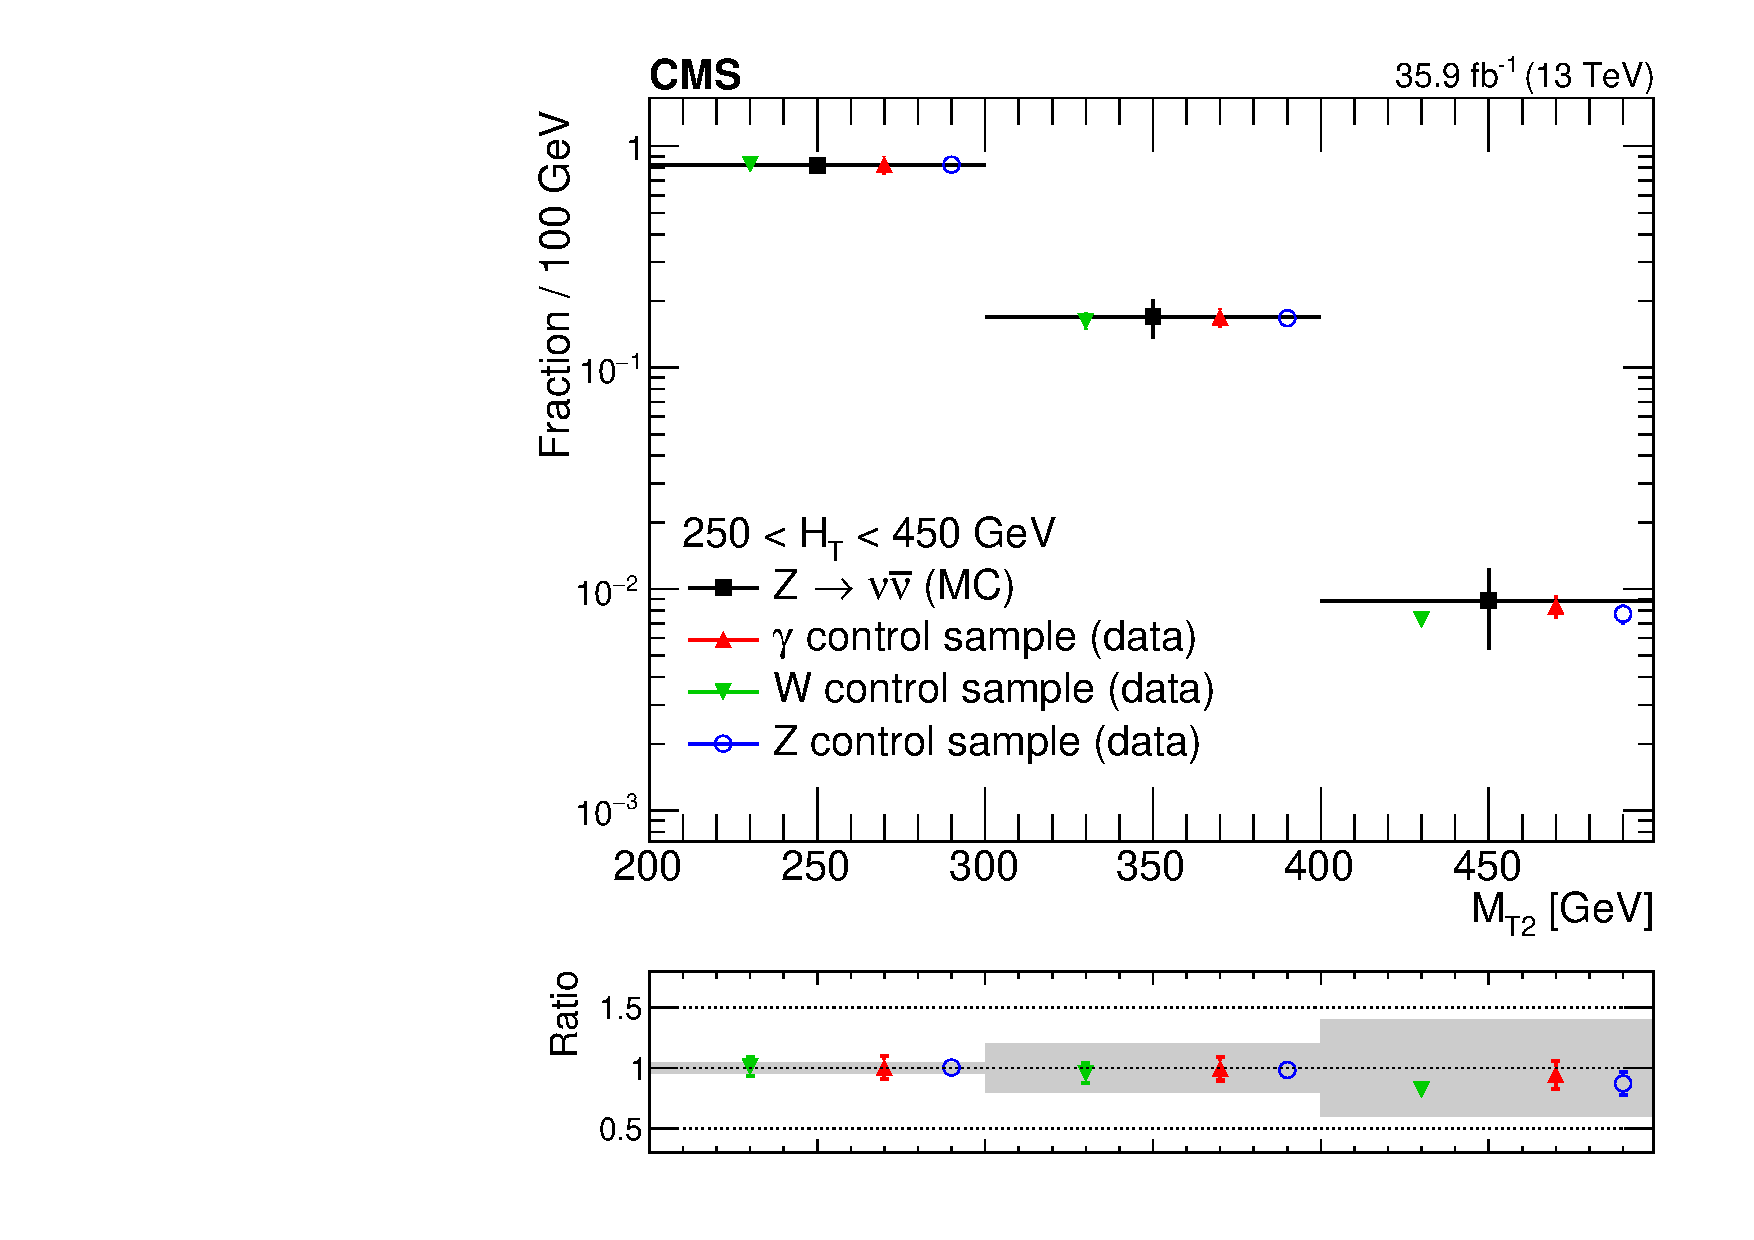
\includegraphics[width=0.35\textwidth]{backgrounds/figs/MT2VL_W_GJ_log}
	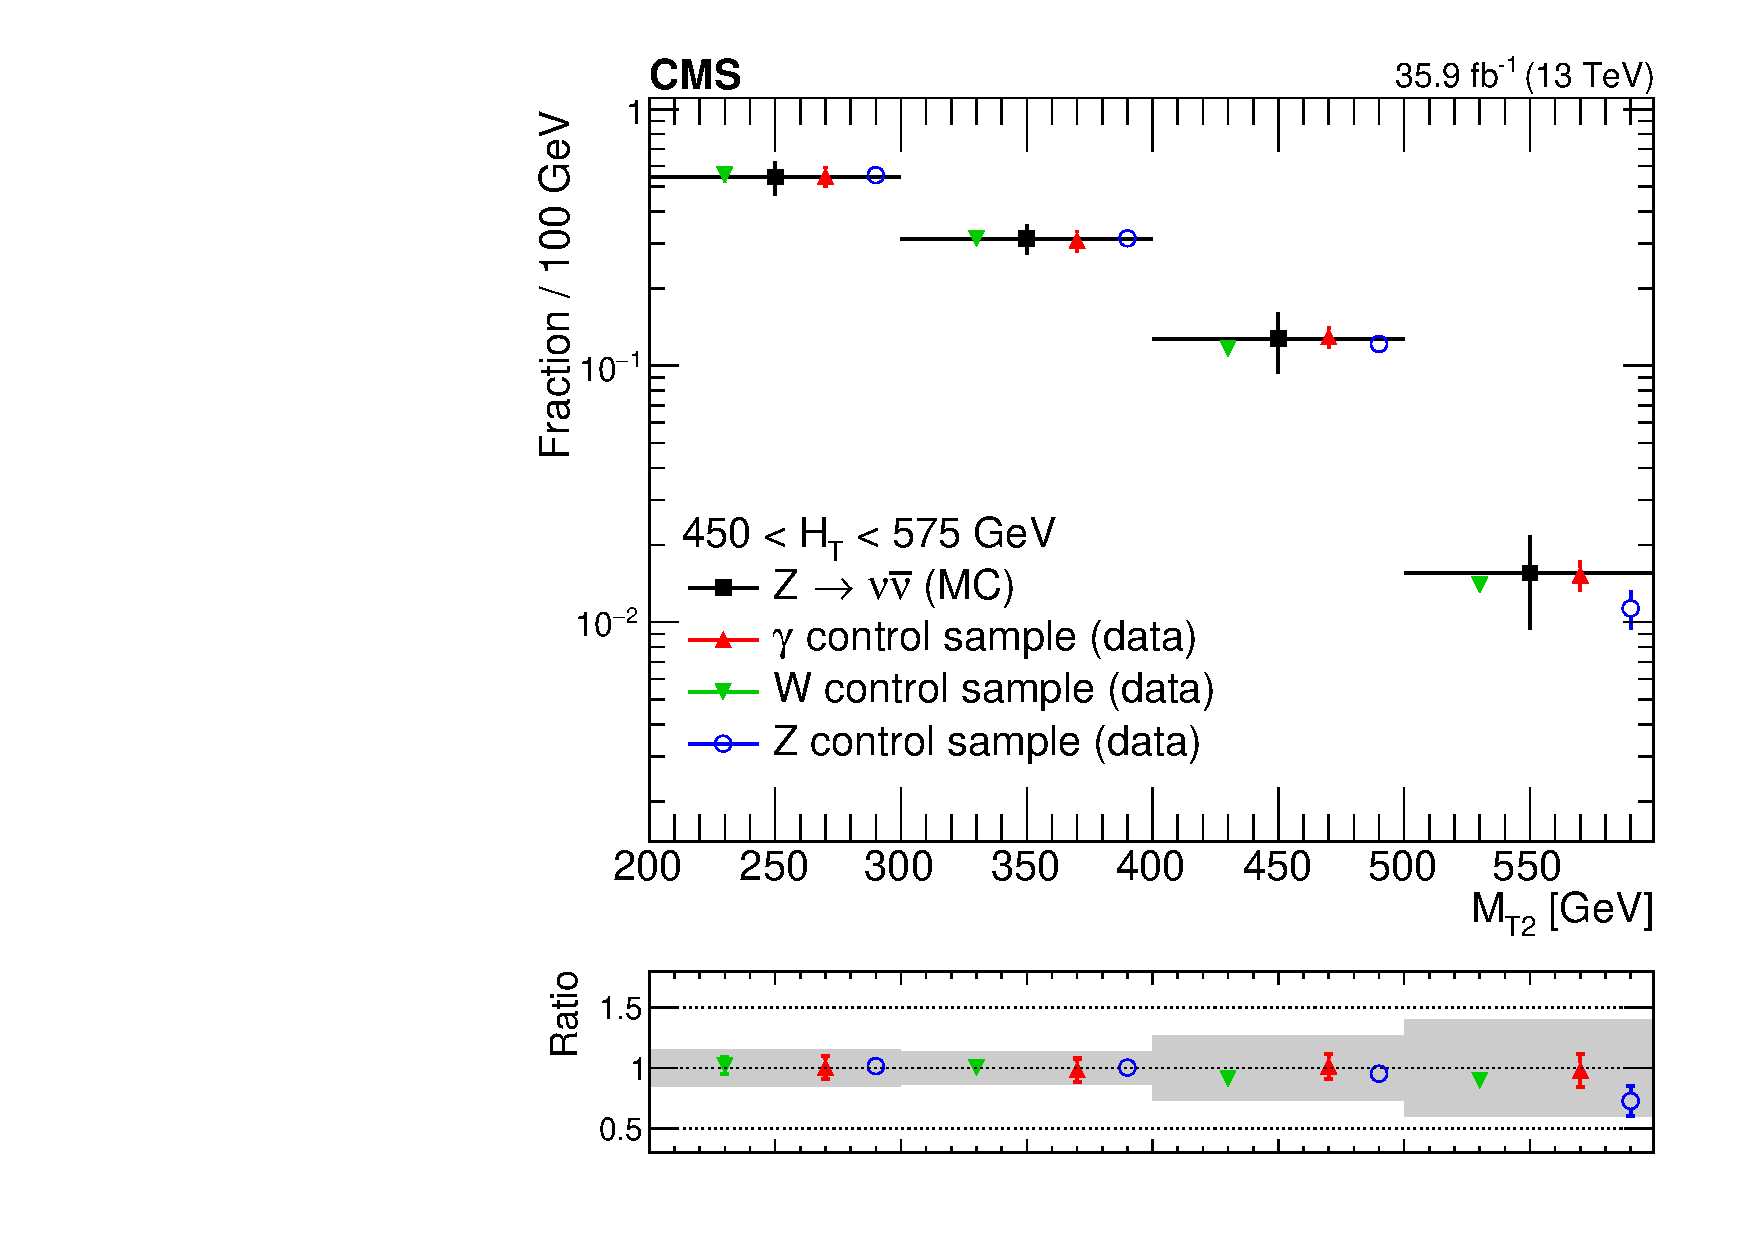
\includegraphics[width=0.35\textwidth]{backgrounds/figs/MT2L_W_GJ_log}
	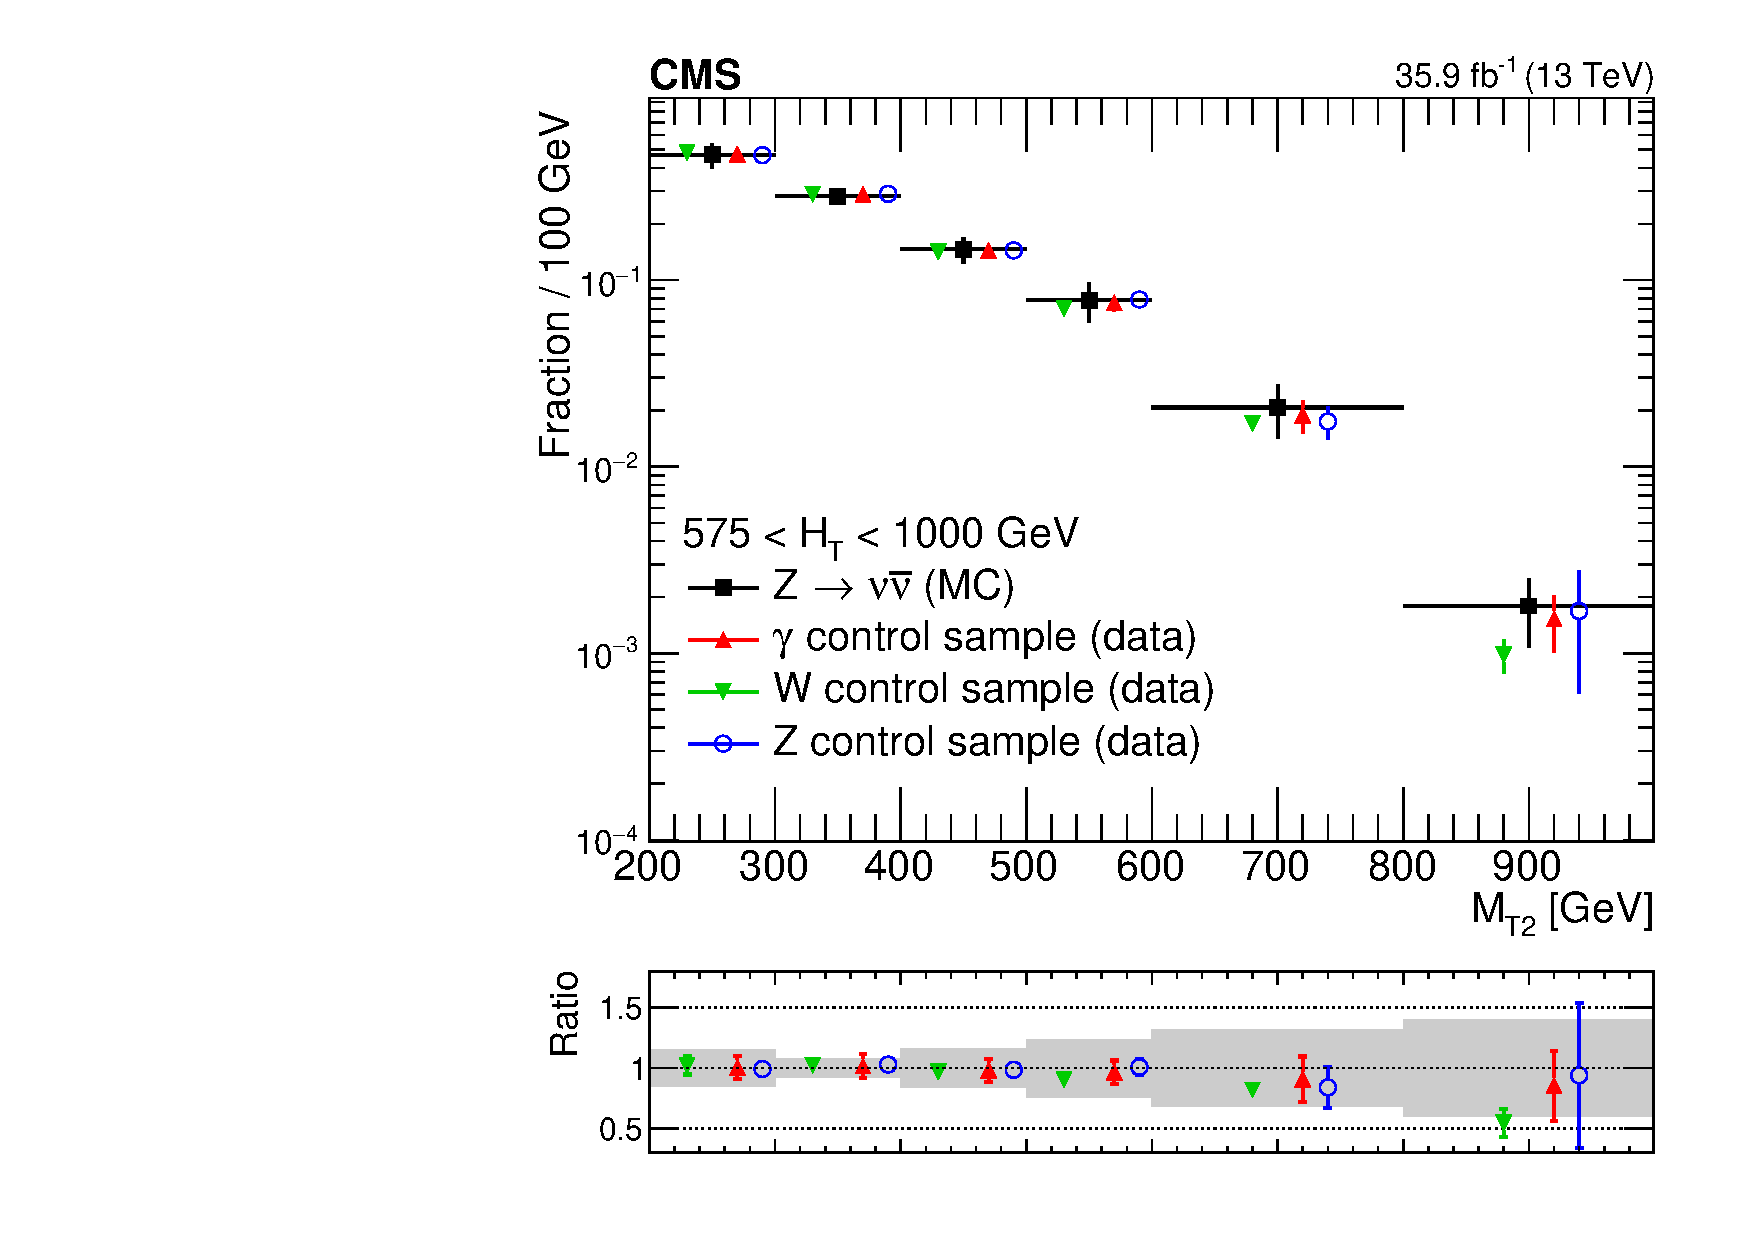
\includegraphics[width=0.35\textwidth]{backgrounds/figs/MT2M_W_GJ_log}
	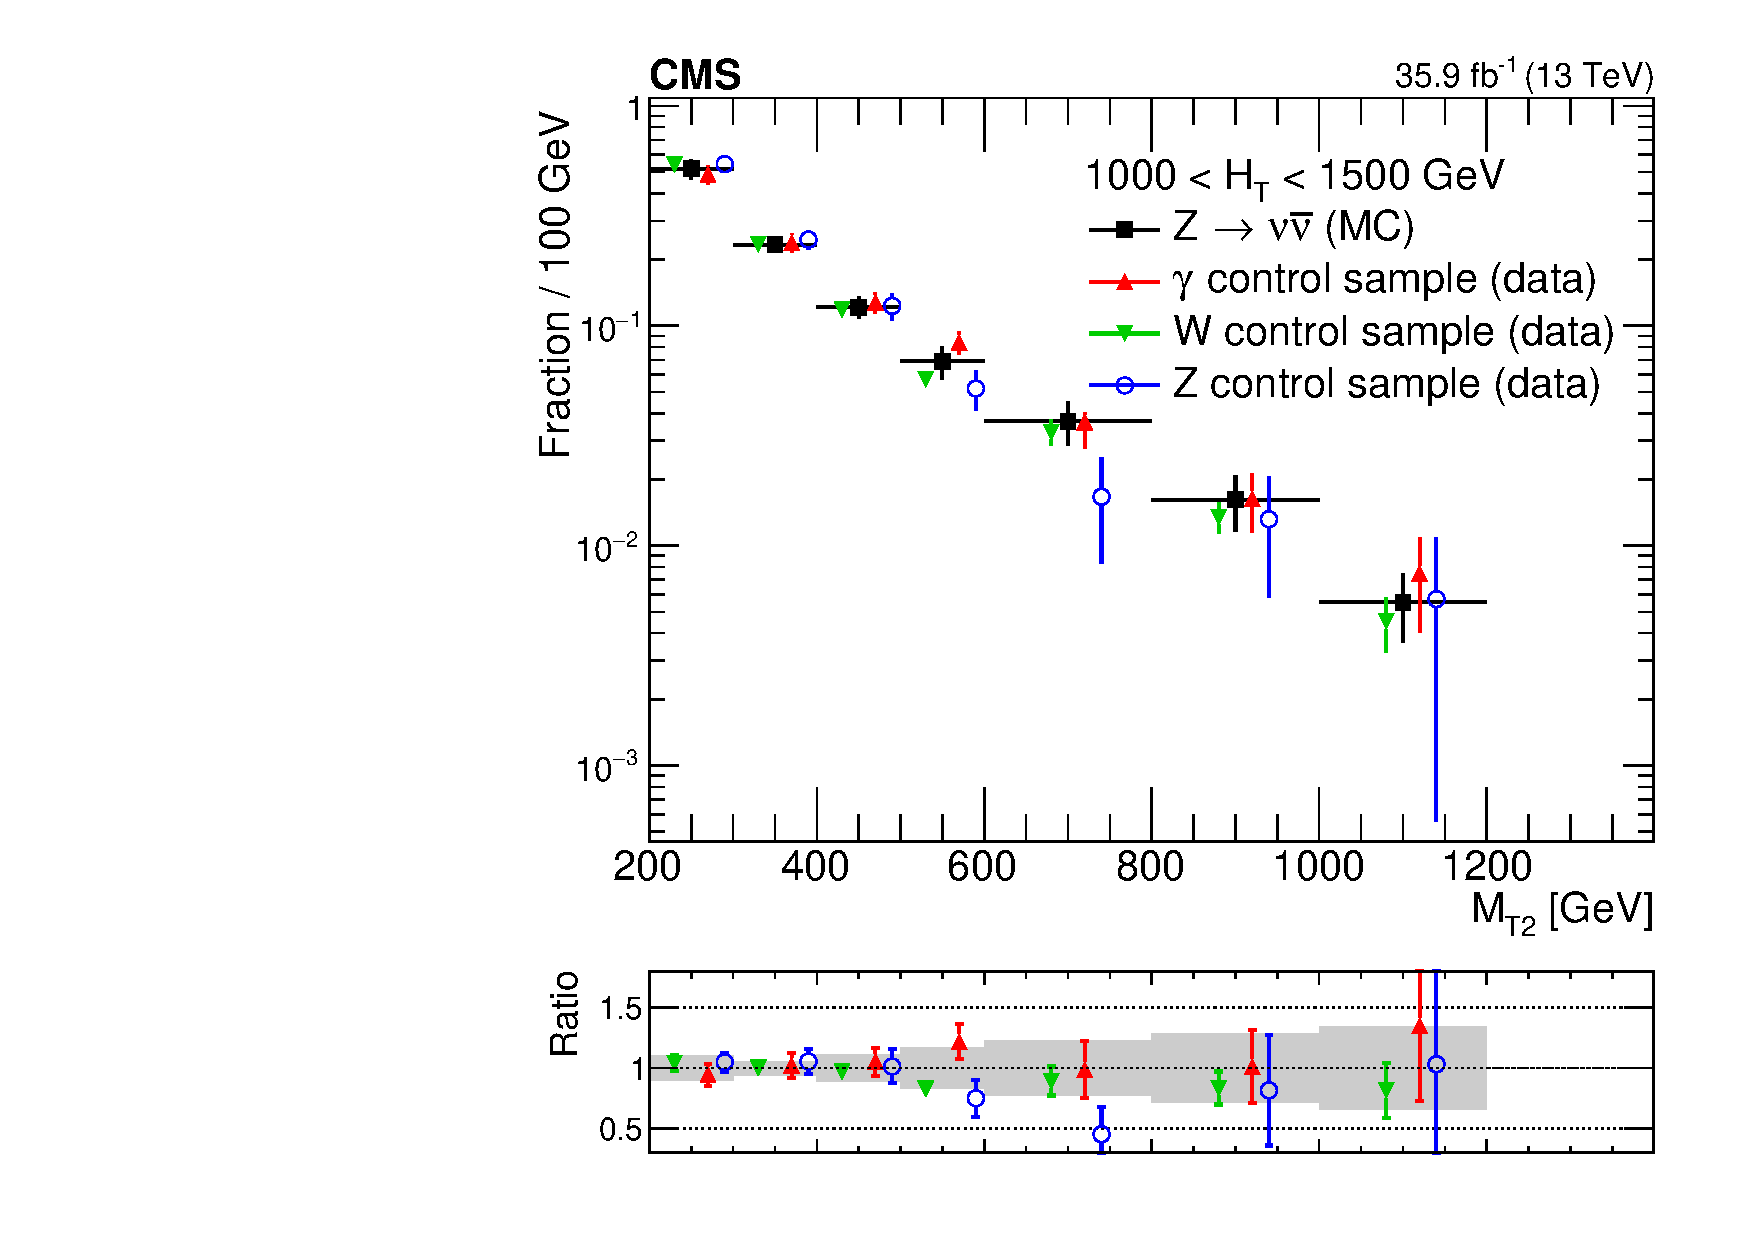
\includegraphics[width=0.35\textwidth]{backgrounds/figs/MT2H_W_GJ_log}
	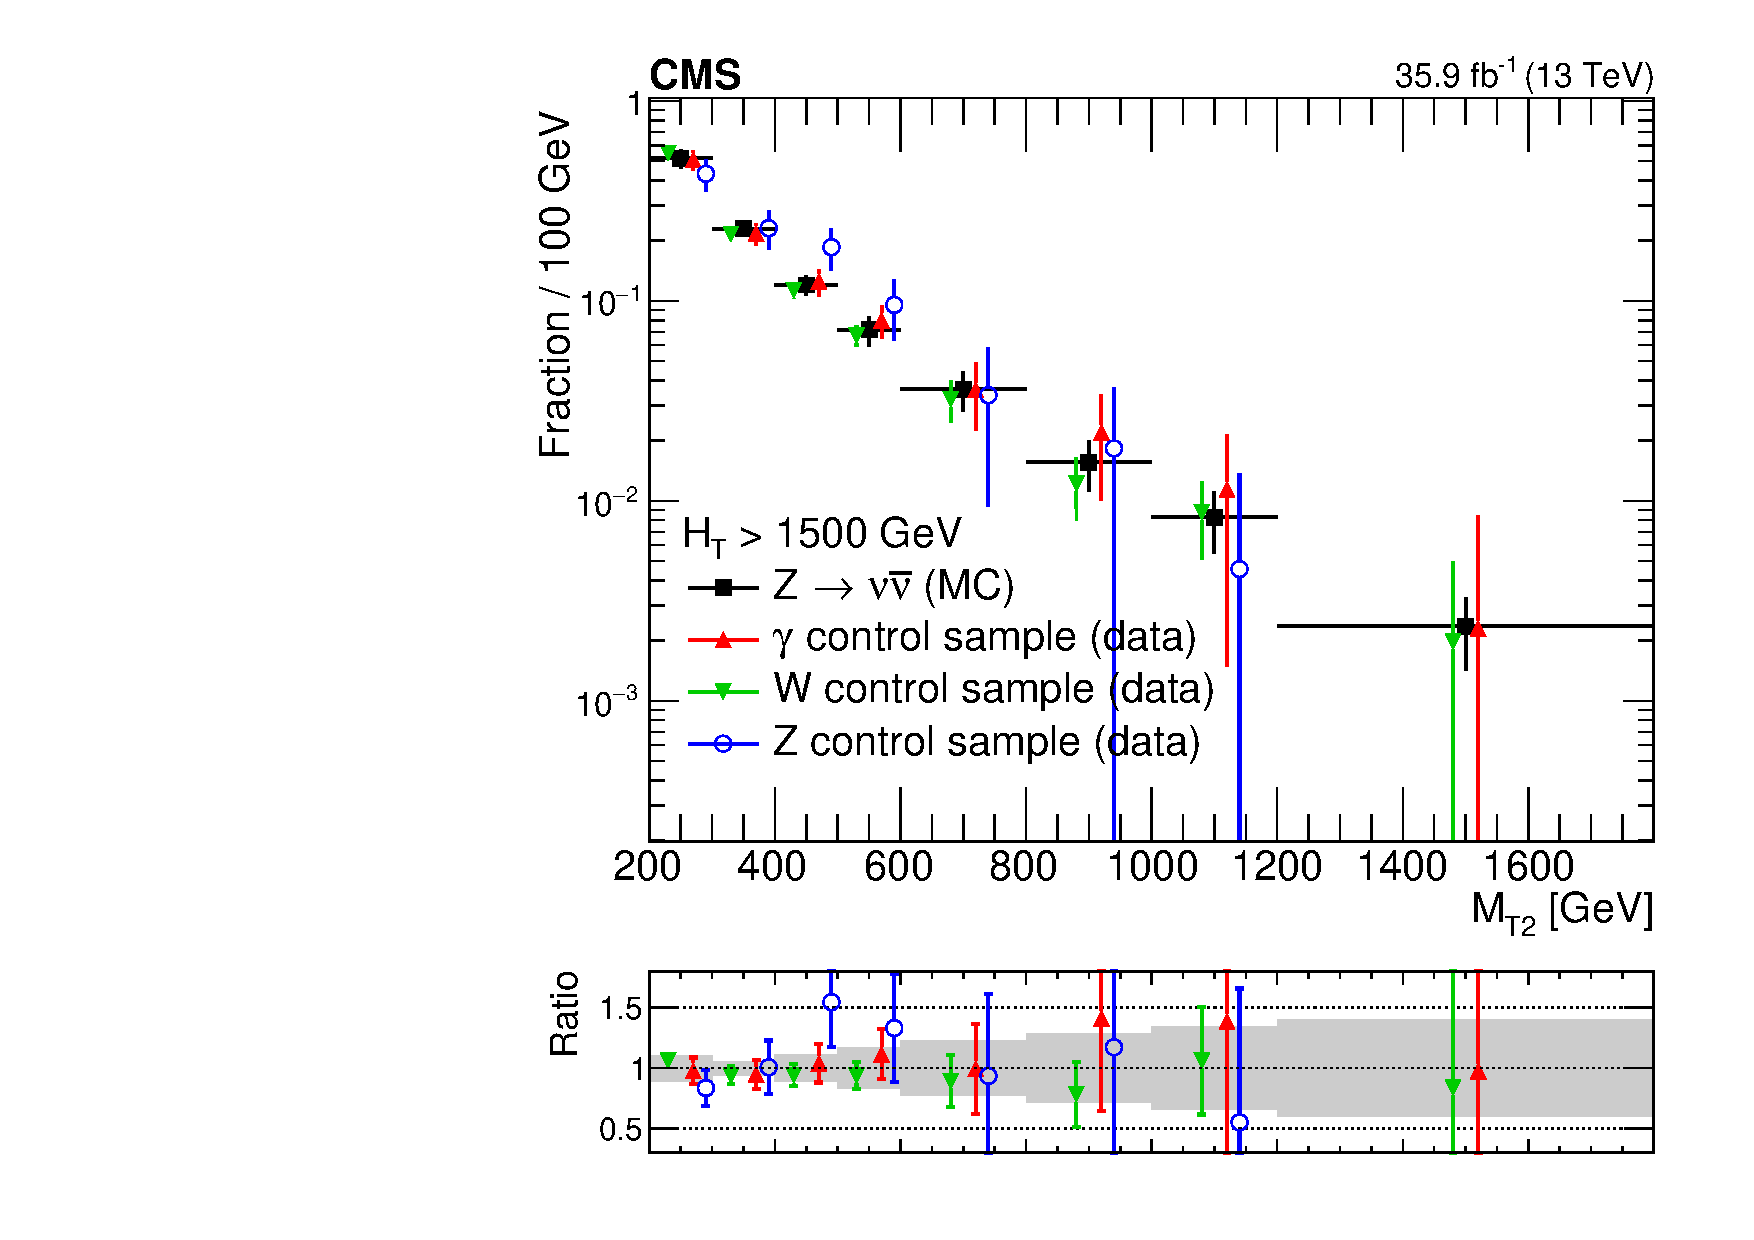
\includegraphics[width=0.35\textwidth]{backgrounds/figs/MT2UH_W_GJ_log}
	\renewcommand{\baselinestretch}{1.0}
	\caption[The \mttwo shape distribution in \znunu simulation compared to $\gamma$, \wlnu, and \zll enriched samples in data, for each \HT region.]{The \mttwo shape distribution in \znunu simulation compared to $\gamma$, \wlnu, and \zll enriched samples in data, for each \HT region. The solid grey band indicates the systematic uncertainty associated with the \mttwo shape modeling.}
	\label{fig:zinvMt2Shape}
\end{figure}

\subsection{Systematic Uncertainties}
\label{subsec:zinvSyst}

Several sources of uncertainty are assessed for the invisible Z estimate, including those associated with the various transfer factors and the \mttwo shape modeling in simulation. The dominant uncertainty in regions using an \mttwo template constructed from data is the statistics of the template. The full list of systematic uncertainties is as follows:
\begin{itemize}
	\item {\it Control region statistical error:} the Poisson error on the number of observed events in \zll data is taken as an uncorrelated uncertainty across all signal regions.
	\item {\it $R_{\mathrm{MC}}^{\znunu/\zll}$ statistical error:} the statistical error associated with the number of MC events generated factors into the transfer factor.
	\item {\it $R_{\mathrm{MC}}^{\znunu/\zll}$ systematic error:} a 5.5\% uncertainty based on variations of lepton efficiency uncertainties as well as other modeling parameters (jet energy scales, factorization and renormalization scales, etc.) is applied as a correlated error in each topological region.
	\item {\it Flavor-symmetric subtraction statistical error:} a Poisson error based on the number of observed opposite-flavor events.
	\item {\it Flavor-symmetric subtraction systematic error:} a 15\% uncertainty on the \ttbar contamination based on the $R^{\mathrm{SF/OF}}$ uncertainty.
	\item {\it \mttwo shape uncertainty:} in regions where the simulation is used to model the \mttwo distribution, additional variations of the renormalization and factorization scales, parton distribution functions, b-tagging scale factor uncertainties, and jet energy scale uncertainties are performed to measure their effect on the \mttwo shape modeling. The most significant impact is seen in the highest \mttwo bins of up to 20\%. In order to cover the uncertainty from additional electro-weak corrections not present in simulation (and possibly not covered by the above variations), a conservative upper threshold of 40\% is used, and the shape uncertainty (in regions where MC \mttwo shape modeling is used) is assigned as a linear morphing of the \mttwo shape starting in the first bin from which MC extrapolation is used, growing to 40\% in the final bin. The shape morphing in every distinct topological region is taken as an uncorrelated error.
	
\end{itemize}


% --------------------------------------------------------------------------- %
% --------------------------------------------------------------------------- %


This chapter makes use of figures and tables from the \mttwo paper and internal analysis note to illustrate the analysis design, methodology, and results. This work was made possible by contributions from the rest of the Surf \& Turf group, our collaborators at ETH Zurich, and the many other CMS members in the SUSY group and beyond.

% --------------------------------------------------------------------------- %
% --------------------------------------------------------------------------- %
